\documentclass[twoside]{book}

% Packages required by doxygen
\usepackage{fixltx2e}
\usepackage{calc}
\usepackage{doxygen}
\usepackage[export]{adjustbox} % also loads graphicx
\usepackage{graphicx}
\usepackage[utf8]{inputenc}
\usepackage{makeidx}
\usepackage{multicol}
\usepackage{multirow}
\PassOptionsToPackage{warn}{textcomp}
\usepackage{textcomp}
\usepackage[nointegrals]{wasysym}
\usepackage[table]{xcolor}

% Font selection
\usepackage[T1]{fontenc}
\usepackage[scaled=.90]{helvet}
\usepackage{courier}
\usepackage{amssymb}
\usepackage{sectsty}
\renewcommand{\familydefault}{\sfdefault}
\allsectionsfont{%
  \fontseries{bc}\selectfont%
  \color{darkgray}%
}
\renewcommand{\DoxyLabelFont}{%
  \fontseries{bc}\selectfont%
  \color{darkgray}%
}
\newcommand{\+}{\discretionary{\mbox{\scriptsize$\hookleftarrow$}}{}{}}

% Page & text layout
\usepackage{geometry}
\geometry{%
  a4paper,%
  top=2.5cm,%
  bottom=2.5cm,%
  left=2.5cm,%
  right=2.5cm%
}
\tolerance=750
\hfuzz=15pt
\hbadness=750
\setlength{\emergencystretch}{15pt}
\setlength{\parindent}{0cm}
\setlength{\parskip}{3ex plus 2ex minus 2ex}
\makeatletter
\renewcommand{\paragraph}{%
  \@startsection{paragraph}{4}{0ex}{-1.0ex}{1.0ex}{%
    \normalfont\normalsize\bfseries\SS@parafont%
  }%
}
\renewcommand{\subparagraph}{%
  \@startsection{subparagraph}{5}{0ex}{-1.0ex}{1.0ex}{%
    \normalfont\normalsize\bfseries\SS@subparafont%
  }%
}
\makeatother

% Headers & footers
\usepackage{fancyhdr}
\pagestyle{fancyplain}
\fancyhead[LE]{\fancyplain{}{\bfseries\thepage}}
\fancyhead[CE]{\fancyplain{}{}}
\fancyhead[RE]{\fancyplain{}{\bfseries\leftmark}}
\fancyhead[LO]{\fancyplain{}{\bfseries\rightmark}}
\fancyhead[CO]{\fancyplain{}{}}
\fancyhead[RO]{\fancyplain{}{\bfseries\thepage}}
\fancyfoot[LE]{\fancyplain{}{}}
\fancyfoot[CE]{\fancyplain{}{}}
\fancyfoot[RE]{\fancyplain{}{\bfseries\scriptsize Generated by Doxygen }}
\fancyfoot[LO]{\fancyplain{}{\bfseries\scriptsize Generated by Doxygen }}
\fancyfoot[CO]{\fancyplain{}{}}
\fancyfoot[RO]{\fancyplain{}{}}
\renewcommand{\footrulewidth}{0.4pt}
\renewcommand{\chaptermark}[1]{%
  \markboth{#1}{}%
}
\renewcommand{\sectionmark}[1]{%
  \markright{\thesection\ #1}%
}

% Indices & bibliography
\usepackage{natbib}
\usepackage[titles]{tocloft}
\setcounter{tocdepth}{3}
\setcounter{secnumdepth}{5}
\makeindex

% Hyperlinks (required, but should be loaded last)
\usepackage{ifpdf}
\ifpdf
  \usepackage[pdftex,pagebackref=true]{hyperref}
\else
  \usepackage[ps2pdf,pagebackref=true]{hyperref}
\fi
\hypersetup{%
  colorlinks=true,%
  linkcolor=blue,%
  citecolor=blue,%
  unicode%
}

% Custom commands
\newcommand{\clearemptydoublepage}{%
  \newpage{\pagestyle{empty}\cleardoublepage}%
}

\usepackage{caption}
\captionsetup{labelsep=space,justification=centering,font={bf},singlelinecheck=off,skip=4pt,position=top}

%===== C O N T E N T S =====

\begin{document}

% Titlepage & ToC
\hypersetup{pageanchor=false,
             bookmarksnumbered=true,
             pdfencoding=unicode
            }
\pagenumbering{roman}
\begin{titlepage}
\vspace*{7cm}
\begin{center}%
{\Large P\+A\+P\+\_\+\+P\+R\+O\+J\+E\+KT \\[1ex]\large 1.\+1 }\\
\vspace*{1cm}
{\large Generated by Doxygen 1.8.11}\\
\end{center}
\end{titlepage}
\clearemptydoublepage
\tableofcontents
\clearemptydoublepage
\pagenumbering{arabic}
\hypersetup{pageanchor=true}

%--- Begin generated contents ---
\chapter{Programowanie aplikacji klient-\/serwer -\/ Wykresy próbek}
\label{index}\hypertarget{index}{}\begin{DoxyAuthor}{Authors}
Mateusz Rzeczkowski 

Krzysztof Kozoń
\end{DoxyAuthor}
\begin{DoxyDate}{Date}
11.\+07.\+2018
\end{DoxyDate}
Aplikacja składa się z klienta i serwera napisanych w C. Klient wysyła do serwera plik zawierający próbki pobierane z urządzenia pomiarowego w równych odstępach czasu (parametr konfigurowalny). Serwer na tej podstawie tworzy wykres pomiarów wykorzystując aplikację do rysowania (np. gnuplot), eksportuje go do pliku i przesyła klientowi. Komunikacja zabezpieczona jest za pomocą Open\+S\+SL.\hypertarget{index_s1}{}\section{Dokumentacja użytkownika}\label{index_s1}
\hypertarget{index_ss1}{}\subsection{Serwer}\label{index_ss1}
Należy uruchomić serwer poprzez uruchomienie pliku ./\+P\+L\+O\+T\+T\+E\+R\+\_\+\+S\+E\+R\+V\+ER z konsoli systemowej. Po uruchomieniu sie, serwer poprosi o haslo certyfikatu, ktore należy podac. W przypadku bledu nalezy sie upewnic czy wpisywane haslo jest poprawne.\hypertarget{index_ss2}{}\subsection{Klient}\label{index_ss2}
Należy uruchomić klienta poprzez uruchomienie pliku ./\+P\+L\+O\+T\+T\+E\+R\+\_\+\+C\+L\+I\+E\+NT z konsoli systemowej, dodatkowo jako argument można podać ścieżkę do pliku, który chcemy przeslac (domyślnie plik nie wiekszy niz 8kB). Po przeslaniu pliku serwer odpowie odsylajac wykres. 
\chapter{File Index}
\section{File List}
Here is a list of all files with brief descriptions\+:\begin{DoxyCompactList}
\item\contentsline{section}{/home/mint/\+Desktop/\+P\+A\+P\+\_\+\+P\+R\+O\+J\+E\+K\+T/\hyperlink{_p_l_o_t_t_e_r___c_l_i_e_n_t_8c}{P\+L\+O\+T\+T\+E\+R\+\_\+\+C\+L\+I\+E\+N\+T.\+c} }{\pageref{_p_l_o_t_t_e_r___c_l_i_e_n_t_8c}}{}
\item\contentsline{section}{/home/mint/\+Desktop/\+P\+A\+P\+\_\+\+P\+R\+O\+J\+E\+K\+T/\hyperlink{_p_l_o_t_t_e_r___s_e_r_v_e_r_8c}{P\+L\+O\+T\+T\+E\+R\+\_\+\+S\+E\+R\+V\+E\+R.\+c} }{\pageref{_p_l_o_t_t_e_r___s_e_r_v_e_r_8c}}{}
\item\contentsline{section}{/home/mint/\+Desktop/\+P\+A\+P\+\_\+\+P\+R\+O\+J\+E\+K\+T/\hyperlink{_project_lib_8h}{Project\+Lib.\+h} }{\pageref{_project_lib_8h}}{}
\item\contentsline{section}{/home/mint/\+Desktop/\+P\+A\+P\+\_\+\+P\+R\+O\+J\+E\+K\+T/\hyperlink{_s_s_l___f_u_n_c_t_i_o_n_s_8h}{S\+S\+L\+\_\+\+F\+U\+N\+C\+T\+I\+O\+N\+S.\+h} }{\pageref{_s_s_l___f_u_n_c_t_i_o_n_s_8h}}{}
\item\contentsline{section}{/home/mint/\+Desktop/\+P\+A\+P\+\_\+\+P\+R\+O\+J\+E\+K\+T/client\+Files/\hyperlink{_client_lib_8h}{Client\+Lib.\+h} }{\pageref{_client_lib_8h}}{}
\item\contentsline{section}{/home/mint/\+Desktop/\+P\+A\+P\+\_\+\+P\+R\+O\+J\+E\+K\+T/doxy/\hyperlink{docmain_8c}{docmain.\+c} }{\pageref{docmain_8c}}{}
\item\contentsline{section}{/home/mint/\+Desktop/\+P\+A\+P\+\_\+\+P\+R\+O\+J\+E\+K\+T/server\+Files/\hyperlink{_server_lib_8h}{Server\+Lib.\+h} }{\pageref{_server_lib_8h}}{}
\end{DoxyCompactList}

\chapter{File Documentation}
\hypertarget{_client_lib_8h}{}\section{/home/mint/\+Desktop/\+P\+A\+P\+\_\+\+P\+R\+O\+J\+E\+K\+T/client\+Files/\+Client\+Lib.h File Reference}
\label{_client_lib_8h}\index{/home/mint/\+Desktop/\+P\+A\+P\+\_\+\+P\+R\+O\+J\+E\+K\+T/client\+Files/\+Client\+Lib.\+h@{/home/mint/\+Desktop/\+P\+A\+P\+\_\+\+P\+R\+O\+J\+E\+K\+T/client\+Files/\+Client\+Lib.\+h}}
{\ttfamily \#include \char`\"{}../\+S\+S\+L\+\_\+\+F\+U\+N\+C\+T\+I\+O\+N\+S.\+h\char`\"{}}\\*
{\ttfamily \#include $<$time.\+h$>$}\\*
Include dependency graph for Client\+Lib.\+h\+:\nopagebreak
\begin{figure}[H]
\begin{center}
\leavevmode
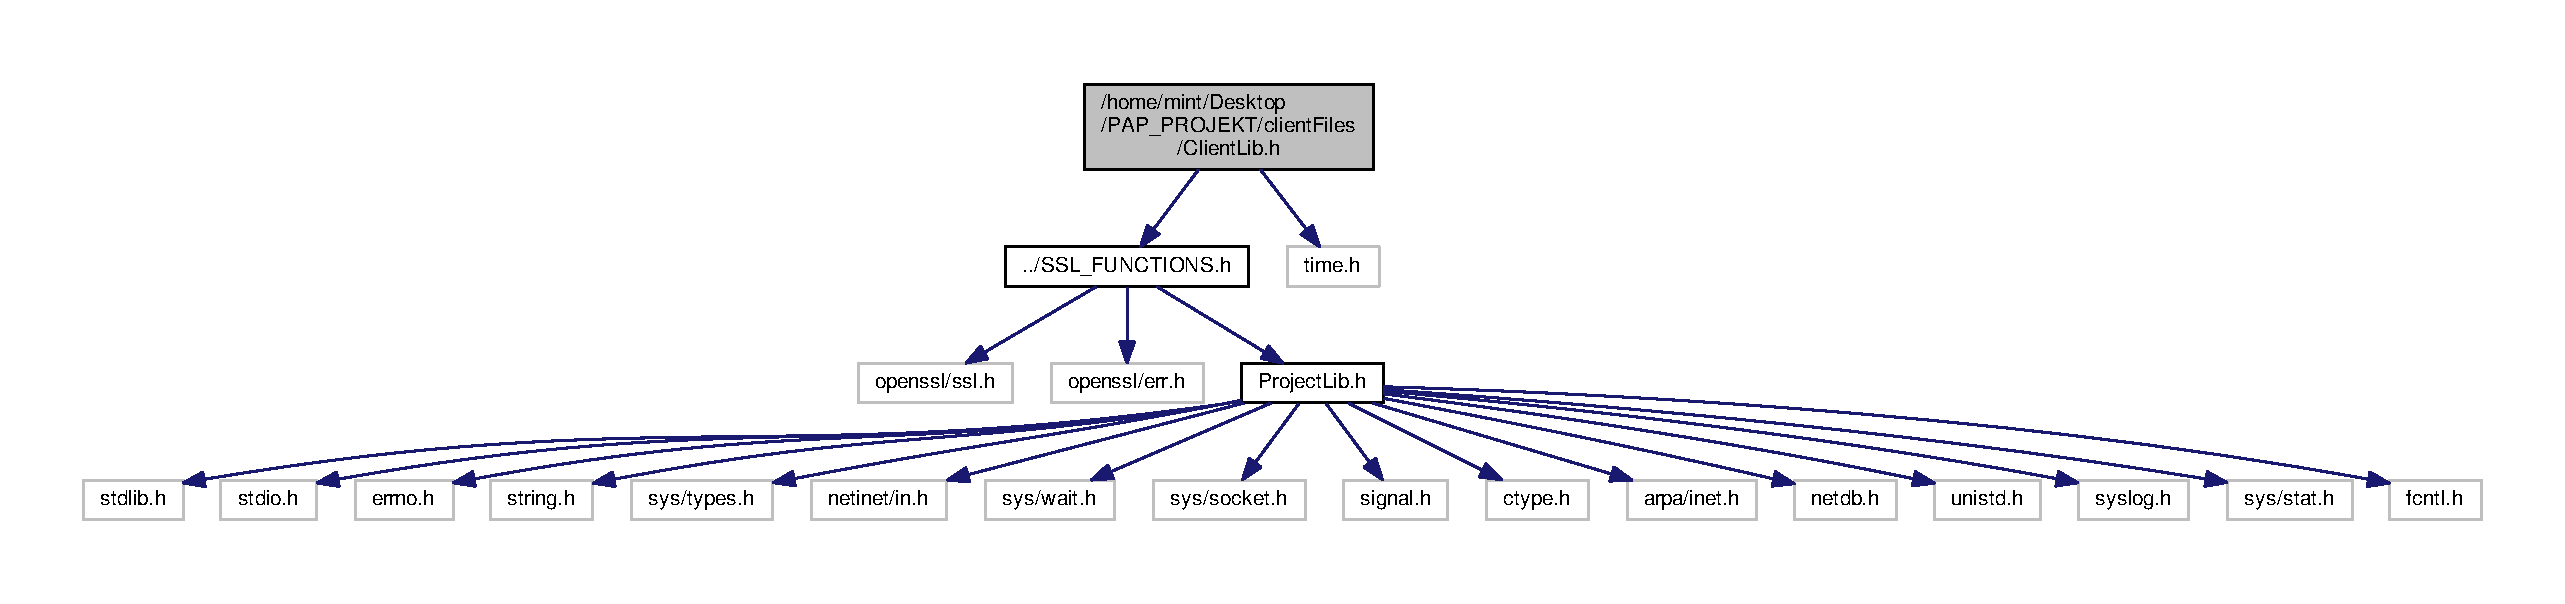
\includegraphics[width=350pt]{_client_lib_8h__incl}
\end{center}
\end{figure}
This graph shows which files directly or indirectly include this file\+:\nopagebreak
\begin{figure}[H]
\begin{center}
\leavevmode
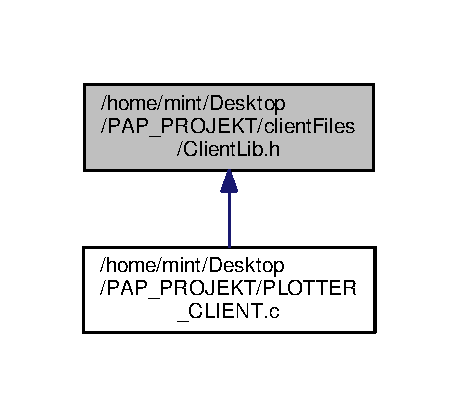
\includegraphics[width=220pt]{_client_lib_8h__dep__incl}
\end{center}
\end{figure}
\subsection*{Functions}
\begin{DoxyCompactItemize}
\item 
void \hyperlink{_client_lib_8h_af6522c0bf90112d406d555fc980f6ae9}{Send\+File\+To\+Server} (char $\ast$\hyperlink{_server_lib_8h_ad5334765c4af576144103e5bfea9b01e}{fs\+\_\+name})
\item 
void \hyperlink{_client_lib_8h_ad453af427d2a8dca1bbca7898ef9ad04}{Receive\+File\+From\+Server} (char $\ast$\hyperlink{_server_lib_8h_a136e211133c7af859abfc129f4e950fa}{fr\+\_\+name})
\item 
void \hyperlink{_client_lib_8h_a1863a0101fe9f7732423c00ae1b64dbc}{Connect\+With\+Port} (int \hyperlink{_p_l_o_t_t_e_r___s_e_r_v_e_r_8c_a614217d263be1fb1a5f76e2ff7be19a2}{P\+O\+RT})
\item 
static int \hyperlink{_client_lib_8h_afa61945039a6813d1d3807080be55a60}{Get\+Client\+Socket\+FD} ()
\item 
static void \hyperlink{_client_lib_8h_a931157773e5116d217f9f79438589dc6}{Close\+Client\+Connection} ()
\end{DoxyCompactItemize}
\subsection*{Variables}
\begin{DoxyCompactItemize}
\item 
static S\+S\+L\+\_\+\+M\+E\+T\+H\+OD $\ast$ \hyperlink{_client_lib_8h_a67a0b3150dfacb2f75fba66e0959f560}{client\+\_\+ssl\+\_\+method}
\begin{DoxyCompactList}\small\item\em Describes the ssl library functions which implement the protocol version. \end{DoxyCompactList}\item 
static S\+S\+L\+\_\+\+C\+TX $\ast$ \hyperlink{_client_lib_8h_ae5429a87dee8628ab5a51bdcb88e336a}{client\+\_\+ssl\+\_\+ctx}
\begin{DoxyCompactList}\small\item\em The global context structure. \end{DoxyCompactList}\item 
static S\+SL $\ast$ \hyperlink{_client_lib_8h_a29a4fb7a75bd99073cdf6a6c871ad771}{client\+\_\+ssl}
\begin{DoxyCompactList}\small\item\em Core structure in the S\+SL A\+PI. \end{DoxyCompactList}\item 
static int \hyperlink{_client_lib_8h_ad2c8fb3df3a737e0685e902870a611d2}{sockfd}
\begin{DoxyCompactList}\small\item\em Socket file descriptor. \end{DoxyCompactList}\end{DoxyCompactItemize}


\subsection{Function Documentation}
\index{Client\+Lib.\+h@{Client\+Lib.\+h}!Close\+Client\+Connection@{Close\+Client\+Connection}}
\index{Close\+Client\+Connection@{Close\+Client\+Connection}!Client\+Lib.\+h@{Client\+Lib.\+h}}
\subsubsection[{\texorpdfstring{Close\+Client\+Connection()}{CloseClientConnection()}}]{\setlength{\rightskip}{0pt plus 5cm}static void Close\+Client\+Connection (
\begin{DoxyParamCaption}
{}
\end{DoxyParamCaption}
)\hspace{0.3cm}{\ttfamily [static]}}\hypertarget{_client_lib_8h_a931157773e5116d217f9f79438589dc6}{}\label{_client_lib_8h_a931157773e5116d217f9f79438589dc6}
Closes a connection with Server 

Definition at line 79 of file Client\+Lib.\+h.

\index{Client\+Lib.\+h@{Client\+Lib.\+h}!Connect\+With\+Port@{Connect\+With\+Port}}
\index{Connect\+With\+Port@{Connect\+With\+Port}!Client\+Lib.\+h@{Client\+Lib.\+h}}
\subsubsection[{\texorpdfstring{Connect\+With\+Port(int P\+O\+R\+T)}{ConnectWithPort(int PORT)}}]{\setlength{\rightskip}{0pt plus 5cm}void Connect\+With\+Port (
\begin{DoxyParamCaption}
\item[{int}]{P\+O\+RT}
\end{DoxyParamCaption}
)}\hypertarget{_client_lib_8h_a1863a0101fe9f7732423c00ae1b64dbc}{}\label{_client_lib_8h_a1863a0101fe9f7732423c00ae1b64dbc}
Connects with server 

Definition at line 32 of file Client\+Lib.\+h.

\index{Client\+Lib.\+h@{Client\+Lib.\+h}!Get\+Client\+Socket\+FD@{Get\+Client\+Socket\+FD}}
\index{Get\+Client\+Socket\+FD@{Get\+Client\+Socket\+FD}!Client\+Lib.\+h@{Client\+Lib.\+h}}
\subsubsection[{\texorpdfstring{Get\+Client\+Socket\+F\+D()}{GetClientSocketFD()}}]{\setlength{\rightskip}{0pt plus 5cm}int Get\+Client\+Socket\+FD (
\begin{DoxyParamCaption}
{}
\end{DoxyParamCaption}
)\hspace{0.3cm}{\ttfamily [static]}}\hypertarget{_client_lib_8h_afa61945039a6813d1d3807080be55a60}{}\label{_client_lib_8h_afa61945039a6813d1d3807080be55a60}
Return a socket file descriptor 

Definition at line 18 of file Client\+Lib.\+h.

\index{Client\+Lib.\+h@{Client\+Lib.\+h}!Receive\+File\+From\+Server@{Receive\+File\+From\+Server}}
\index{Receive\+File\+From\+Server@{Receive\+File\+From\+Server}!Client\+Lib.\+h@{Client\+Lib.\+h}}
\subsubsection[{\texorpdfstring{Receive\+File\+From\+Server(char $\ast$fr\+\_\+name)}{ReceiveFileFromServer(char *fr_name)}}]{\setlength{\rightskip}{0pt plus 5cm}void Receive\+File\+From\+Server (
\begin{DoxyParamCaption}
\item[{char $\ast$}]{fr\+\_\+name}
\end{DoxyParamCaption}
)}\hypertarget{_client_lib_8h_ad453af427d2a8dca1bbca7898ef9ad04}{}\label{_client_lib_8h_ad453af427d2a8dca1bbca7898ef9ad04}
Gets plot image form the server 

Definition at line 69 of file Client\+Lib.\+h.

\index{Client\+Lib.\+h@{Client\+Lib.\+h}!Send\+File\+To\+Server@{Send\+File\+To\+Server}}
\index{Send\+File\+To\+Server@{Send\+File\+To\+Server}!Client\+Lib.\+h@{Client\+Lib.\+h}}
\subsubsection[{\texorpdfstring{Send\+File\+To\+Server(char $\ast$fs\+\_\+name)}{SendFileToServer(char *fs_name)}}]{\setlength{\rightskip}{0pt plus 5cm}void Send\+File\+To\+Server (
\begin{DoxyParamCaption}
\item[{char $\ast$}]{fs\+\_\+name}
\end{DoxyParamCaption}
)}\hypertarget{_client_lib_8h_af6522c0bf90112d406d555fc980f6ae9}{}\label{_client_lib_8h_af6522c0bf90112d406d555fc980f6ae9}
Sends data to the server that will be plotted 

Definition at line 59 of file Client\+Lib.\+h.



\subsection{Variable Documentation}
\index{Client\+Lib.\+h@{Client\+Lib.\+h}!client\+\_\+ssl@{client\+\_\+ssl}}
\index{client\+\_\+ssl@{client\+\_\+ssl}!Client\+Lib.\+h@{Client\+Lib.\+h}}
\subsubsection[{\texorpdfstring{client\+\_\+ssl}{client_ssl}}]{\setlength{\rightskip}{0pt plus 5cm}S\+SL$\ast$ client\+\_\+ssl\hspace{0.3cm}{\ttfamily [static]}}\hypertarget{_client_lib_8h_a29a4fb7a75bd99073cdf6a6c871ad771}{}\label{_client_lib_8h_a29a4fb7a75bd99073cdf6a6c871ad771}


Core structure in the S\+SL A\+PI. 



Definition at line 13 of file Client\+Lib.\+h.

\index{Client\+Lib.\+h@{Client\+Lib.\+h}!client\+\_\+ssl\+\_\+ctx@{client\+\_\+ssl\+\_\+ctx}}
\index{client\+\_\+ssl\+\_\+ctx@{client\+\_\+ssl\+\_\+ctx}!Client\+Lib.\+h@{Client\+Lib.\+h}}
\subsubsection[{\texorpdfstring{client\+\_\+ssl\+\_\+ctx}{client_ssl_ctx}}]{\setlength{\rightskip}{0pt plus 5cm}S\+S\+L\+\_\+\+C\+TX$\ast$ client\+\_\+ssl\+\_\+ctx\hspace{0.3cm}{\ttfamily [static]}}\hypertarget{_client_lib_8h_ae5429a87dee8628ab5a51bdcb88e336a}{}\label{_client_lib_8h_ae5429a87dee8628ab5a51bdcb88e336a}


The global context structure. 



Definition at line 12 of file Client\+Lib.\+h.

\index{Client\+Lib.\+h@{Client\+Lib.\+h}!client\+\_\+ssl\+\_\+method@{client\+\_\+ssl\+\_\+method}}
\index{client\+\_\+ssl\+\_\+method@{client\+\_\+ssl\+\_\+method}!Client\+Lib.\+h@{Client\+Lib.\+h}}
\subsubsection[{\texorpdfstring{client\+\_\+ssl\+\_\+method}{client_ssl_method}}]{\setlength{\rightskip}{0pt plus 5cm}S\+S\+L\+\_\+\+M\+E\+T\+H\+OD$\ast$ client\+\_\+ssl\+\_\+method\hspace{0.3cm}{\ttfamily [static]}}\hypertarget{_client_lib_8h_a67a0b3150dfacb2f75fba66e0959f560}{}\label{_client_lib_8h_a67a0b3150dfacb2f75fba66e0959f560}


Describes the ssl library functions which implement the protocol version. 



Definition at line 11 of file Client\+Lib.\+h.

\index{Client\+Lib.\+h@{Client\+Lib.\+h}!sockfd@{sockfd}}
\index{sockfd@{sockfd}!Client\+Lib.\+h@{Client\+Lib.\+h}}
\subsubsection[{\texorpdfstring{sockfd}{sockfd}}]{\setlength{\rightskip}{0pt plus 5cm}int sockfd\hspace{0.3cm}{\ttfamily [static]}}\hypertarget{_client_lib_8h_ad2c8fb3df3a737e0685e902870a611d2}{}\label{_client_lib_8h_ad2c8fb3df3a737e0685e902870a611d2}


Socket file descriptor. 



Definition at line 15 of file Client\+Lib.\+h.


\hypertarget{docmain_8c}{}\section{/home/mint/\+Desktop/\+P\+A\+P\+\_\+\+P\+R\+O\+J\+E\+K\+T/doxy/docmain.c File Reference}
\label{docmain_8c}\index{/home/mint/\+Desktop/\+P\+A\+P\+\_\+\+P\+R\+O\+J\+E\+K\+T/doxy/docmain.\+c@{/home/mint/\+Desktop/\+P\+A\+P\+\_\+\+P\+R\+O\+J\+E\+K\+T/doxy/docmain.\+c}}

\hypertarget{_p_l_o_t_t_e_r___c_l_i_e_n_t_8c}{}\section{/home/mint/\+Desktop/\+P\+A\+P\+\_\+\+P\+R\+O\+J\+E\+K\+T/\+P\+L\+O\+T\+T\+E\+R\+\_\+\+C\+L\+I\+E\+NT.c File Reference}
\label{_p_l_o_t_t_e_r___c_l_i_e_n_t_8c}\index{/home/mint/\+Desktop/\+P\+A\+P\+\_\+\+P\+R\+O\+J\+E\+K\+T/\+P\+L\+O\+T\+T\+E\+R\+\_\+\+C\+L\+I\+E\+N\+T.\+c@{/home/mint/\+Desktop/\+P\+A\+P\+\_\+\+P\+R\+O\+J\+E\+K\+T/\+P\+L\+O\+T\+T\+E\+R\+\_\+\+C\+L\+I\+E\+N\+T.\+c}}
{\ttfamily \#include \char`\"{}client\+Files/\+Client\+Lib.\+h\char`\"{}}\\*
Include dependency graph for P\+L\+O\+T\+T\+E\+R\+\_\+\+C\+L\+I\+E\+N\+T.\+c\+:\nopagebreak
\begin{figure}[H]
\begin{center}
\leavevmode
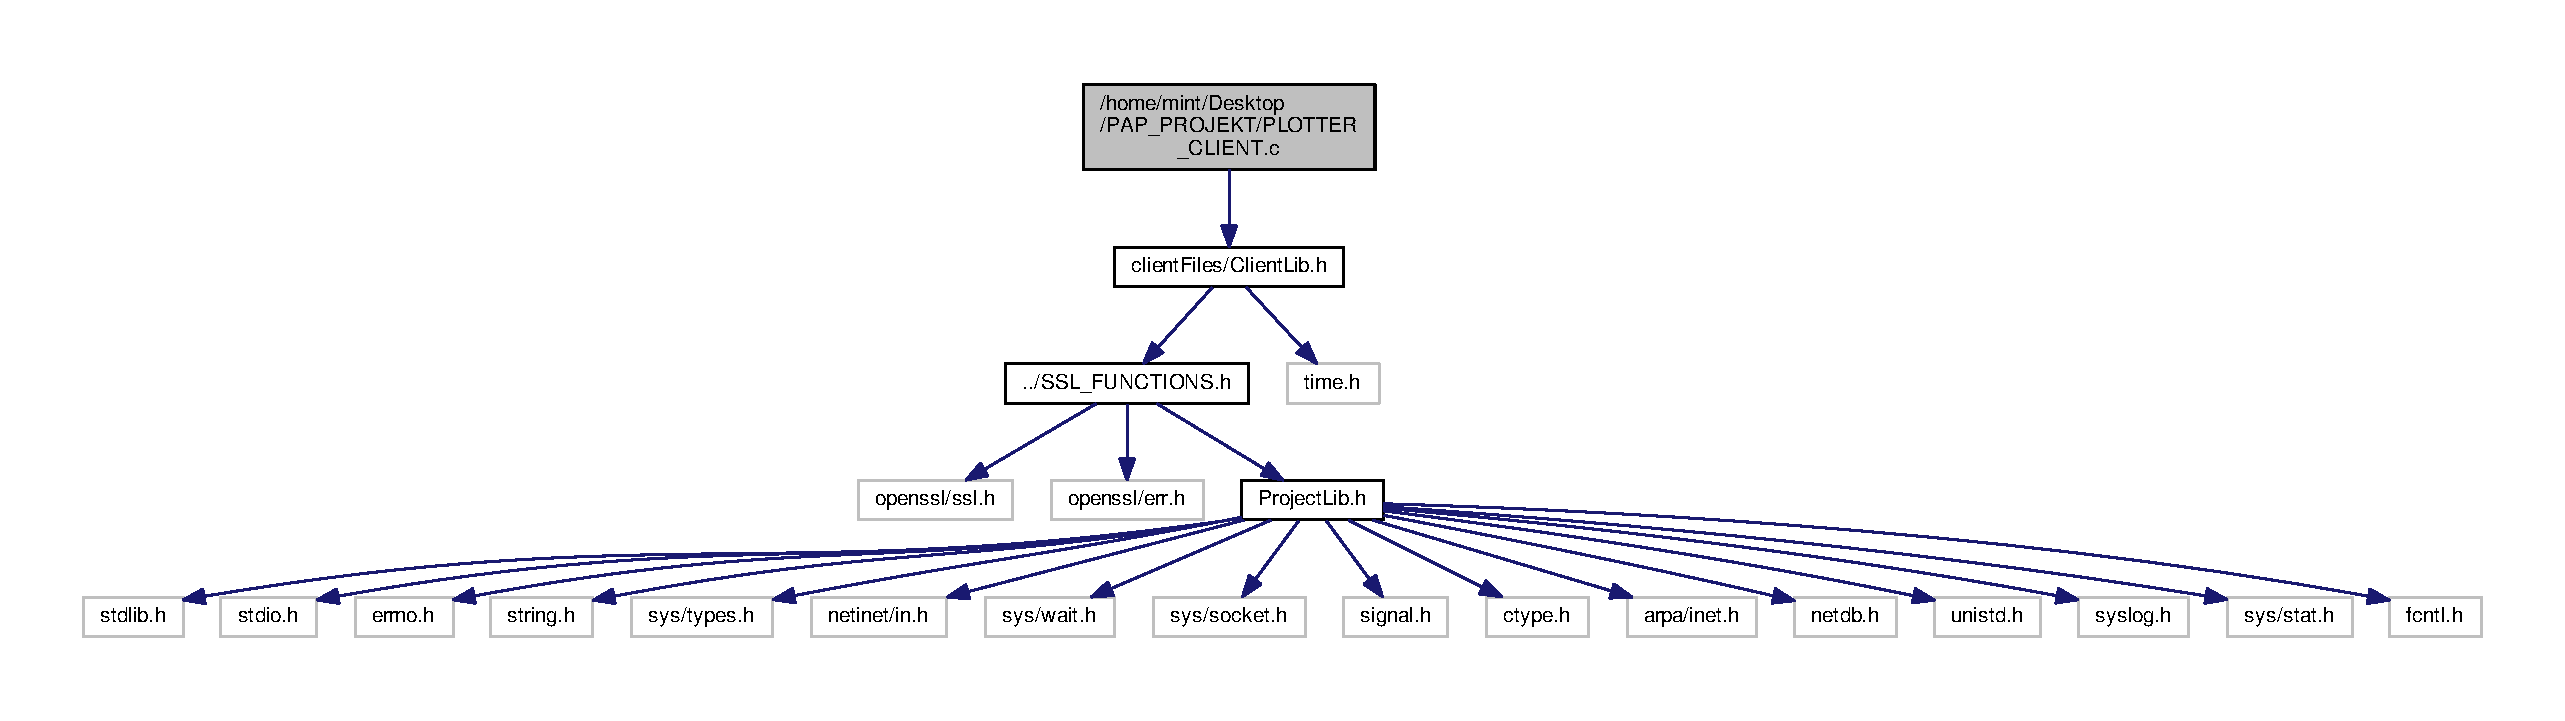
\includegraphics[width=350pt]{_p_l_o_t_t_e_r___c_l_i_e_n_t_8c__incl}
\end{center}
\end{figure}
\subsection*{Macros}
\begin{DoxyCompactItemize}
\item 
\#define \hyperlink{_p_l_o_t_t_e_r___c_l_i_e_n_t_8c_a614217d263be1fb1a5f76e2ff7be19a2}{P\+O\+RT}~5353
\end{DoxyCompactItemize}
\subsection*{Functions}
\begin{DoxyCompactItemize}
\item 
int \hyperlink{_p_l_o_t_t_e_r___c_l_i_e_n_t_8c_a0ddf1224851353fc92bfbff6f499fa97}{main} (int argc, char $\ast$argv\mbox{[}$\,$\mbox{]})
\end{DoxyCompactItemize}


\subsection{Macro Definition Documentation}
\index{P\+L\+O\+T\+T\+E\+R\+\_\+\+C\+L\+I\+E\+N\+T.\+c@{P\+L\+O\+T\+T\+E\+R\+\_\+\+C\+L\+I\+E\+N\+T.\+c}!P\+O\+RT@{P\+O\+RT}}
\index{P\+O\+RT@{P\+O\+RT}!P\+L\+O\+T\+T\+E\+R\+\_\+\+C\+L\+I\+E\+N\+T.\+c@{P\+L\+O\+T\+T\+E\+R\+\_\+\+C\+L\+I\+E\+N\+T.\+c}}
\subsubsection[{\texorpdfstring{P\+O\+RT}{PORT}}]{\setlength{\rightskip}{0pt plus 5cm}\#define P\+O\+RT~5353}\hypertarget{_p_l_o_t_t_e_r___c_l_i_e_n_t_8c_a614217d263be1fb1a5f76e2ff7be19a2}{}\label{_p_l_o_t_t_e_r___c_l_i_e_n_t_8c_a614217d263be1fb1a5f76e2ff7be19a2}


Definition at line 3 of file P\+L\+O\+T\+T\+E\+R\+\_\+\+C\+L\+I\+E\+N\+T.\+c.



\subsection{Function Documentation}
\index{P\+L\+O\+T\+T\+E\+R\+\_\+\+C\+L\+I\+E\+N\+T.\+c@{P\+L\+O\+T\+T\+E\+R\+\_\+\+C\+L\+I\+E\+N\+T.\+c}!main@{main}}
\index{main@{main}!P\+L\+O\+T\+T\+E\+R\+\_\+\+C\+L\+I\+E\+N\+T.\+c@{P\+L\+O\+T\+T\+E\+R\+\_\+\+C\+L\+I\+E\+N\+T.\+c}}
\subsubsection[{\texorpdfstring{main(int argc, char $\ast$argv[])}{main(int argc, char *argv[])}}]{\setlength{\rightskip}{0pt plus 5cm}int main (
\begin{DoxyParamCaption}
\item[{int}]{argc, }
\item[{char $\ast$}]{argv\mbox{[}$\,$\mbox{]}}
\end{DoxyParamCaption}
)}\hypertarget{_p_l_o_t_t_e_r___c_l_i_e_n_t_8c_a0ddf1224851353fc92bfbff6f499fa97}{}\label{_p_l_o_t_t_e_r___c_l_i_e_n_t_8c_a0ddf1224851353fc92bfbff6f499fa97}


Definition at line 5 of file P\+L\+O\+T\+T\+E\+R\+\_\+\+C\+L\+I\+E\+N\+T.\+c.


\hypertarget{_p_l_o_t_t_e_r___s_e_r_v_e_r_8c}{}\section{/home/mint/\+Desktop/\+P\+A\+P\+\_\+\+P\+R\+O\+J\+E\+K\+T/\+P\+L\+O\+T\+T\+E\+R\+\_\+\+S\+E\+R\+V\+ER.c File Reference}
\label{_p_l_o_t_t_e_r___s_e_r_v_e_r_8c}\index{/home/mint/\+Desktop/\+P\+A\+P\+\_\+\+P\+R\+O\+J\+E\+K\+T/\+P\+L\+O\+T\+T\+E\+R\+\_\+\+S\+E\+R\+V\+E\+R.\+c@{/home/mint/\+Desktop/\+P\+A\+P\+\_\+\+P\+R\+O\+J\+E\+K\+T/\+P\+L\+O\+T\+T\+E\+R\+\_\+\+S\+E\+R\+V\+E\+R.\+c}}
{\ttfamily \#include \char`\"{}server\+Files/\+Server\+Lib.\+h\char`\"{}}\\*
Include dependency graph for P\+L\+O\+T\+T\+E\+R\+\_\+\+S\+E\+R\+V\+E\+R.\+c\+:\nopagebreak
\begin{figure}[H]
\begin{center}
\leavevmode
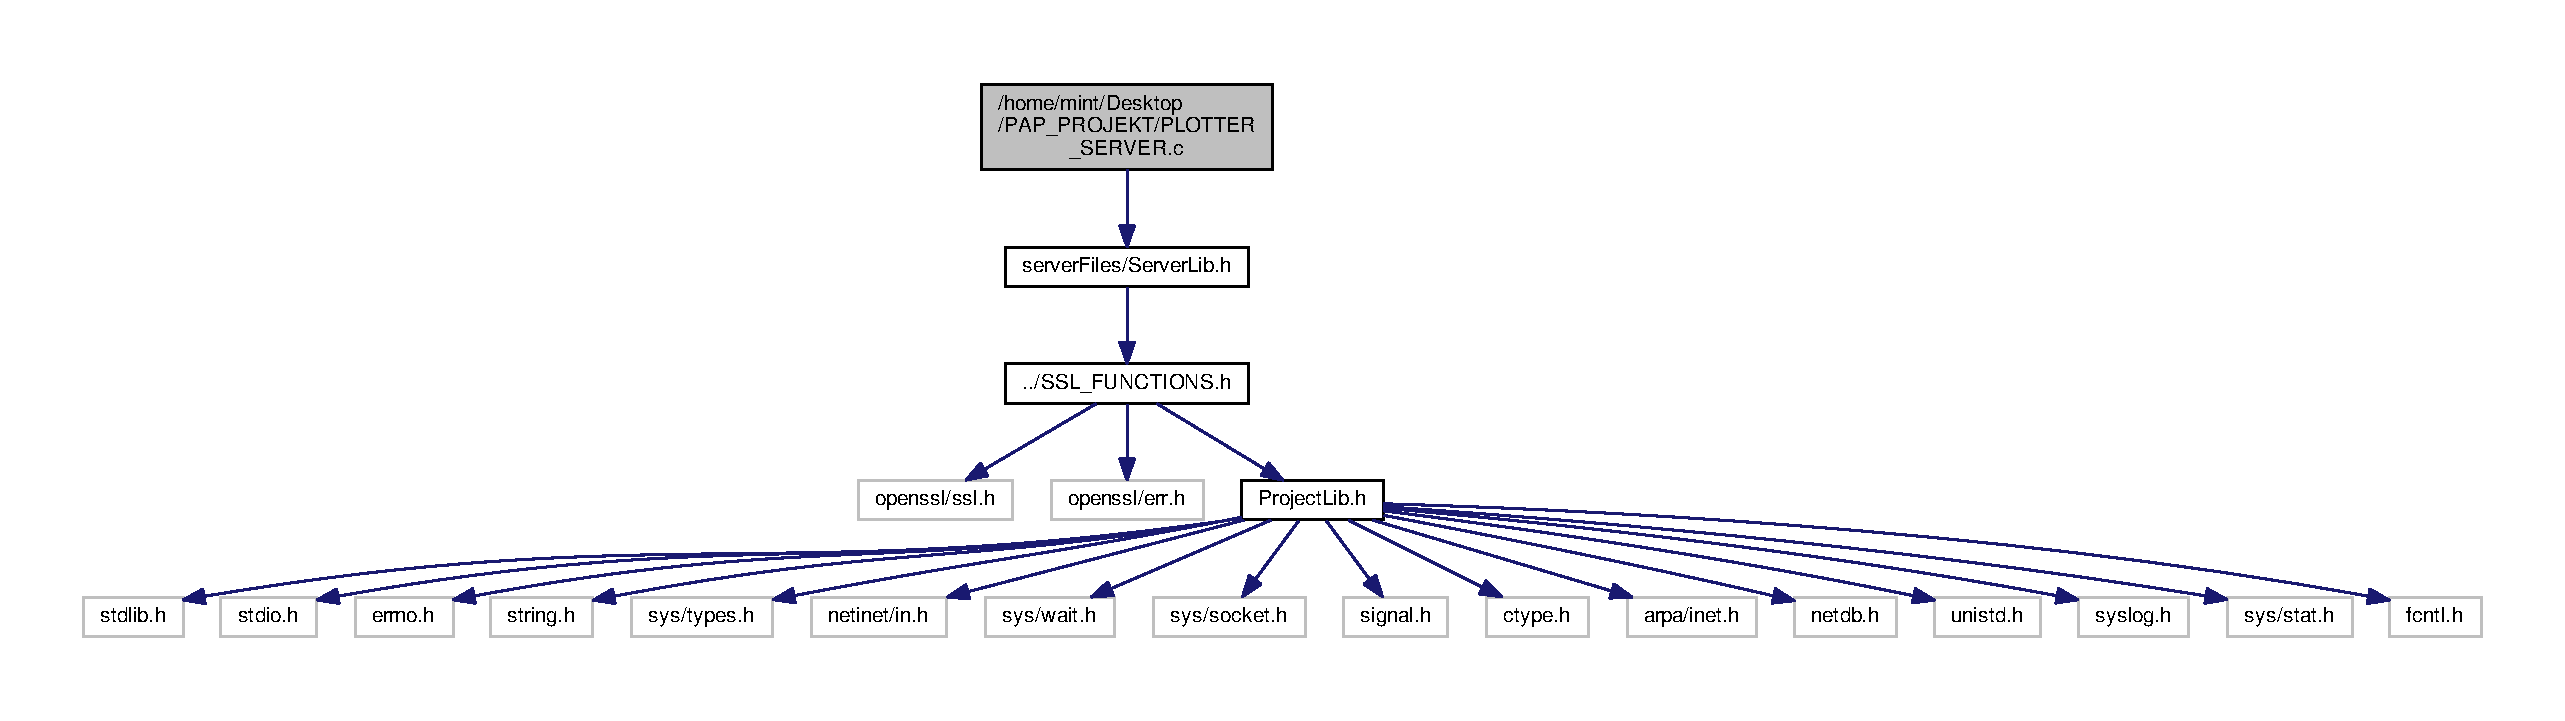
\includegraphics[width=350pt]{_p_l_o_t_t_e_r___s_e_r_v_e_r_8c__incl}
\end{center}
\end{figure}
\subsection*{Macros}
\begin{DoxyCompactItemize}
\item 
\#define \hyperlink{_p_l_o_t_t_e_r___s_e_r_v_e_r_8c_a614217d263be1fb1a5f76e2ff7be19a2}{P\+O\+RT}~5353
\item 
\#define \hyperlink{_p_l_o_t_t_e_r___s_e_r_v_e_r_8c_aeefbbafa97642defe3ee6c3080b7d66f}{B\+A\+C\+K\+L\+OG}~5
\end{DoxyCompactItemize}
\subsection*{Functions}
\begin{DoxyCompactItemize}
\item 
int \hyperlink{_p_l_o_t_t_e_r___s_e_r_v_e_r_8c_a0ddf1224851353fc92bfbff6f499fa97}{main} (int argc, char $\ast$argv\mbox{[}$\,$\mbox{]})
\end{DoxyCompactItemize}


\subsection{Macro Definition Documentation}
\index{P\+L\+O\+T\+T\+E\+R\+\_\+\+S\+E\+R\+V\+E\+R.\+c@{P\+L\+O\+T\+T\+E\+R\+\_\+\+S\+E\+R\+V\+E\+R.\+c}!B\+A\+C\+K\+L\+OG@{B\+A\+C\+K\+L\+OG}}
\index{B\+A\+C\+K\+L\+OG@{B\+A\+C\+K\+L\+OG}!P\+L\+O\+T\+T\+E\+R\+\_\+\+S\+E\+R\+V\+E\+R.\+c@{P\+L\+O\+T\+T\+E\+R\+\_\+\+S\+E\+R\+V\+E\+R.\+c}}
\subsubsection[{\texorpdfstring{B\+A\+C\+K\+L\+OG}{BACKLOG}}]{\setlength{\rightskip}{0pt plus 5cm}\#define B\+A\+C\+K\+L\+OG~5}\hypertarget{_p_l_o_t_t_e_r___s_e_r_v_e_r_8c_aeefbbafa97642defe3ee6c3080b7d66f}{}\label{_p_l_o_t_t_e_r___s_e_r_v_e_r_8c_aeefbbafa97642defe3ee6c3080b7d66f}


Definition at line 4 of file P\+L\+O\+T\+T\+E\+R\+\_\+\+S\+E\+R\+V\+E\+R.\+c.

\index{P\+L\+O\+T\+T\+E\+R\+\_\+\+S\+E\+R\+V\+E\+R.\+c@{P\+L\+O\+T\+T\+E\+R\+\_\+\+S\+E\+R\+V\+E\+R.\+c}!P\+O\+RT@{P\+O\+RT}}
\index{P\+O\+RT@{P\+O\+RT}!P\+L\+O\+T\+T\+E\+R\+\_\+\+S\+E\+R\+V\+E\+R.\+c@{P\+L\+O\+T\+T\+E\+R\+\_\+\+S\+E\+R\+V\+E\+R.\+c}}
\subsubsection[{\texorpdfstring{P\+O\+RT}{PORT}}]{\setlength{\rightskip}{0pt plus 5cm}\#define P\+O\+RT~5353}\hypertarget{_p_l_o_t_t_e_r___s_e_r_v_e_r_8c_a614217d263be1fb1a5f76e2ff7be19a2}{}\label{_p_l_o_t_t_e_r___s_e_r_v_e_r_8c_a614217d263be1fb1a5f76e2ff7be19a2}


Definition at line 3 of file P\+L\+O\+T\+T\+E\+R\+\_\+\+S\+E\+R\+V\+E\+R.\+c.



\subsection{Function Documentation}
\index{P\+L\+O\+T\+T\+E\+R\+\_\+\+S\+E\+R\+V\+E\+R.\+c@{P\+L\+O\+T\+T\+E\+R\+\_\+\+S\+E\+R\+V\+E\+R.\+c}!main@{main}}
\index{main@{main}!P\+L\+O\+T\+T\+E\+R\+\_\+\+S\+E\+R\+V\+E\+R.\+c@{P\+L\+O\+T\+T\+E\+R\+\_\+\+S\+E\+R\+V\+E\+R.\+c}}
\subsubsection[{\texorpdfstring{main(int argc, char $\ast$argv[])}{main(int argc, char *argv[])}}]{\setlength{\rightskip}{0pt plus 5cm}int main (
\begin{DoxyParamCaption}
\item[{int}]{argc, }
\item[{char $\ast$}]{argv\mbox{[}$\,$\mbox{]}}
\end{DoxyParamCaption}
)}\hypertarget{_p_l_o_t_t_e_r___s_e_r_v_e_r_8c_a0ddf1224851353fc92bfbff6f499fa97}{}\label{_p_l_o_t_t_e_r___s_e_r_v_e_r_8c_a0ddf1224851353fc92bfbff6f499fa97}


Definition at line 6 of file P\+L\+O\+T\+T\+E\+R\+\_\+\+S\+E\+R\+V\+E\+R.\+c.


\hypertarget{_project_lib_8h}{}\section{/home/mint/\+Desktop/\+P\+A\+P\+\_\+\+P\+R\+O\+J\+E\+K\+T/\+Project\+Lib.h File Reference}
\label{_project_lib_8h}\index{/home/mint/\+Desktop/\+P\+A\+P\+\_\+\+P\+R\+O\+J\+E\+K\+T/\+Project\+Lib.\+h@{/home/mint/\+Desktop/\+P\+A\+P\+\_\+\+P\+R\+O\+J\+E\+K\+T/\+Project\+Lib.\+h}}
{\ttfamily \#include $<$stdlib.\+h$>$}\\*
{\ttfamily \#include $<$stdio.\+h$>$}\\*
{\ttfamily \#include $<$errno.\+h$>$}\\*
{\ttfamily \#include $<$string.\+h$>$}\\*
{\ttfamily \#include $<$sys/types.\+h$>$}\\*
{\ttfamily \#include $<$netinet/in.\+h$>$}\\*
{\ttfamily \#include $<$sys/wait.\+h$>$}\\*
{\ttfamily \#include $<$sys/socket.\+h$>$}\\*
{\ttfamily \#include $<$signal.\+h$>$}\\*
{\ttfamily \#include $<$ctype.\+h$>$}\\*
{\ttfamily \#include $<$arpa/inet.\+h$>$}\\*
{\ttfamily \#include $<$netdb.\+h$>$}\\*
{\ttfamily \#include $<$unistd.\+h$>$}\\*
{\ttfamily \#include $<$syslog.\+h$>$}\\*
{\ttfamily \#include $<$sys/stat.\+h$>$}\\*
{\ttfamily \#include $<$fcntl.\+h$>$}\\*
Include dependency graph for Project\+Lib.\+h\+:\nopagebreak
\begin{figure}[H]
\begin{center}
\leavevmode
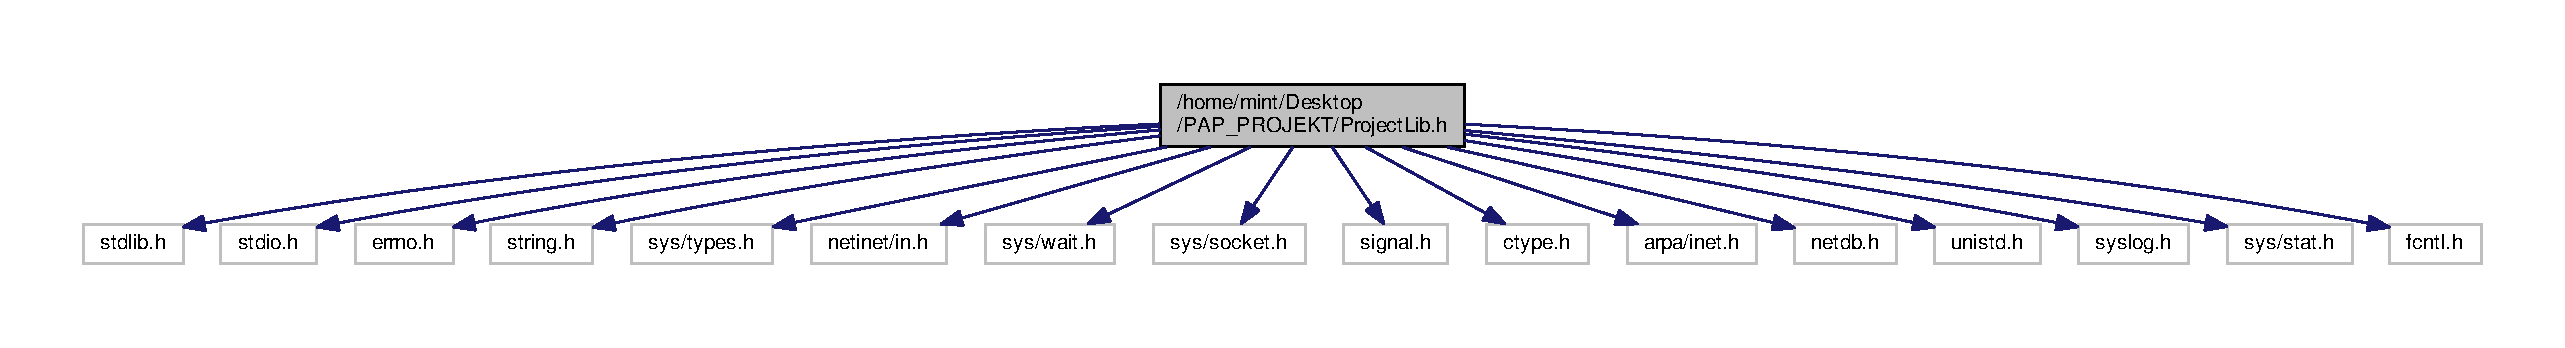
\includegraphics[width=350pt]{_project_lib_8h__incl}
\end{center}
\end{figure}
This graph shows which files directly or indirectly include this file\+:\nopagebreak
\begin{figure}[H]
\begin{center}
\leavevmode
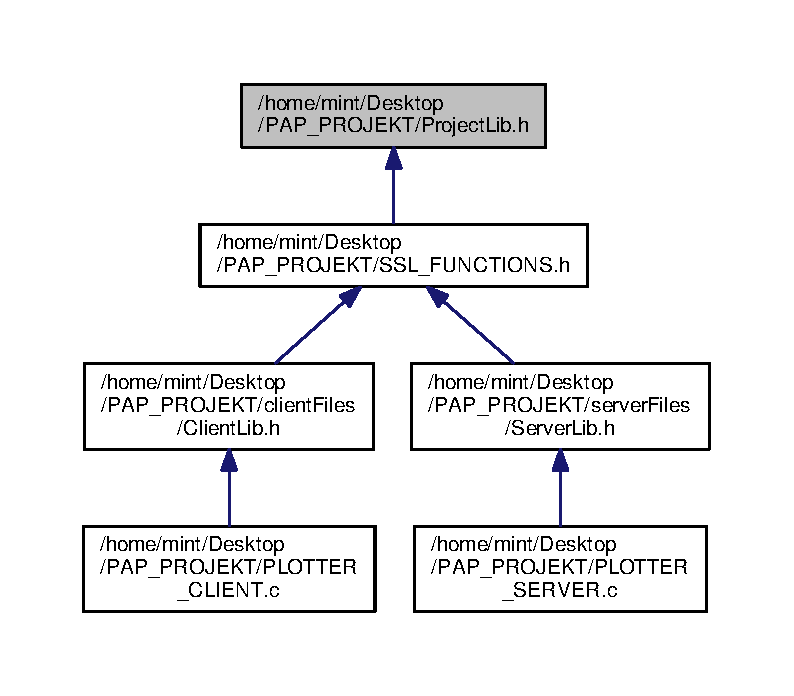
\includegraphics[width=350pt]{_project_lib_8h__dep__incl}
\end{center}
\end{figure}
\subsection*{Macros}
\begin{DoxyCompactItemize}
\item 
\#define \hyperlink{_project_lib_8h_a30362161c93e3f1a4ee4c673f535b5a8}{L\+E\+N\+G\+TH}~8192
\begin{DoxyCompactList}\small\item\em Maximum length of sent file. \end{DoxyCompactList}\end{DoxyCompactItemize}
\subsection*{Functions}
\begin{DoxyCompactItemize}
\item 
void \hyperlink{_project_lib_8h_a7e15c8e2885871839fc2b820dfbdb4ce}{error} ()
\item 
F\+I\+LE $\ast$ \hyperlink{_project_lib_8h_a63d58319cc10a3e1505c56a22bdb0238}{xfopen} (const char $\ast$fn, const char $\ast$mode)
\item 
int \hyperlink{_project_lib_8h_ad32bb943b76f934465207c24f799c9f6}{badmode} (const char $\ast$s)
\item 
int \hyperlink{_project_lib_8h_aea69367c666445568e3215893409419d}{xfclose} (F\+I\+LE $\ast$fp)
\item 
int \hyperlink{_project_lib_8h_a47981aeac52a3ae3da0e30c26266fb7d}{xfexists} (char $\ast$fn)
\item 
char $\ast$ \hyperlink{_project_lib_8h_ac4bf47d0c8ddc34d278f4478d1a0d16d}{fnwoext} (char $\ast$nm, char $\ast$fn)
\end{DoxyCompactItemize}
\subsection*{Variables}
\begin{DoxyCompactItemize}
\item 
char \hyperlink{_project_lib_8h_a179ab0a58242ed797fad4db1a75a4d0f}{err\+Buf} \mbox{[}256\mbox{]}
\begin{DoxyCompactList}\small\item\em The buffer of server errors. \end{DoxyCompactList}\end{DoxyCompactItemize}


\subsection{Macro Definition Documentation}
\index{Project\+Lib.\+h@{Project\+Lib.\+h}!L\+E\+N\+G\+TH@{L\+E\+N\+G\+TH}}
\index{L\+E\+N\+G\+TH@{L\+E\+N\+G\+TH}!Project\+Lib.\+h@{Project\+Lib.\+h}}
\subsubsection[{\texorpdfstring{L\+E\+N\+G\+TH}{LENGTH}}]{\setlength{\rightskip}{0pt plus 5cm}\#define L\+E\+N\+G\+TH~8192}\hypertarget{_project_lib_8h_a30362161c93e3f1a4ee4c673f535b5a8}{}\label{_project_lib_8h_a30362161c93e3f1a4ee4c673f535b5a8}


Maximum length of sent file. 



Definition at line 18 of file Project\+Lib.\+h.



\subsection{Function Documentation}
\index{Project\+Lib.\+h@{Project\+Lib.\+h}!badmode@{badmode}}
\index{badmode@{badmode}!Project\+Lib.\+h@{Project\+Lib.\+h}}
\subsubsection[{\texorpdfstring{badmode(const char $\ast$s)}{badmode(const char *s)}}]{\setlength{\rightskip}{0pt plus 5cm}int badmode (
\begin{DoxyParamCaption}
\item[{const char $\ast$}]{s}
\end{DoxyParamCaption}
)}\hypertarget{_project_lib_8h_ad32bb943b76f934465207c24f799c9f6}{}\label{_project_lib_8h_ad32bb943b76f934465207c24f799c9f6}
Validates file mode \textquotesingle{}s\textquotesingle{} is \char`\"{}rwa+b\char`\"{} 

Definition at line 57 of file Project\+Lib.\+h.

\index{Project\+Lib.\+h@{Project\+Lib.\+h}!error@{error}}
\index{error@{error}!Project\+Lib.\+h@{Project\+Lib.\+h}}
\subsubsection[{\texorpdfstring{error()}{error()}}]{\setlength{\rightskip}{0pt plus 5cm}void error (
\begin{DoxyParamCaption}
{}
\end{DoxyParamCaption}
)}\hypertarget{_project_lib_8h_a7e15c8e2885871839fc2b820dfbdb4ce}{}\label{_project_lib_8h_a7e15c8e2885871839fc2b820dfbdb4ce}
Error reporting function, reports error message that is in err\+Buff 

Definition at line 29 of file Project\+Lib.\+h.

\index{Project\+Lib.\+h@{Project\+Lib.\+h}!fnwoext@{fnwoext}}
\index{fnwoext@{fnwoext}!Project\+Lib.\+h@{Project\+Lib.\+h}}
\subsubsection[{\texorpdfstring{fnwoext(char $\ast$nm, char $\ast$fn)}{fnwoext(char *nm, char *fn)}}]{\setlength{\rightskip}{0pt plus 5cm}char $\ast$ fnwoext (
\begin{DoxyParamCaption}
\item[{char $\ast$}]{nm, }
\item[{char $\ast$}]{fn}
\end{DoxyParamCaption}
)}\hypertarget{_project_lib_8h_ac4bf47d0c8ddc34d278f4478d1a0d16d}{}\label{_project_lib_8h_ac4bf47d0c8ddc34d278f4478d1a0d16d}
Isolates filename, without path or extension 

Definition at line 92 of file Project\+Lib.\+h.

\index{Project\+Lib.\+h@{Project\+Lib.\+h}!xfclose@{xfclose}}
\index{xfclose@{xfclose}!Project\+Lib.\+h@{Project\+Lib.\+h}}
\subsubsection[{\texorpdfstring{xfclose(\+F\+I\+L\+E $\ast$fp)}{xfclose(FILE *fp)}}]{\setlength{\rightskip}{0pt plus 5cm}int xfclose (
\begin{DoxyParamCaption}
\item[{F\+I\+LE $\ast$}]{fp}
\end{DoxyParamCaption}
)}\hypertarget{_project_lib_8h_aea69367c666445568e3215893409419d}{}\label{_project_lib_8h_aea69367c666445568e3215893409419d}
file close with error check 

Definition at line 71 of file Project\+Lib.\+h.

\index{Project\+Lib.\+h@{Project\+Lib.\+h}!xfexists@{xfexists}}
\index{xfexists@{xfexists}!Project\+Lib.\+h@{Project\+Lib.\+h}}
\subsubsection[{\texorpdfstring{xfexists(char $\ast$fn)}{xfexists(char *fn)}}]{\setlength{\rightskip}{0pt plus 5cm}int xfexists (
\begin{DoxyParamCaption}
\item[{char $\ast$}]{fn}
\end{DoxyParamCaption}
)}\hypertarget{_project_lib_8h_a47981aeac52a3ae3da0e30c26266fb7d}{}\label{_project_lib_8h_a47981aeac52a3ae3da0e30c26266fb7d}
Checks if file \textquotesingle{}fn\textquotesingle{} already exists 

Definition at line 82 of file Project\+Lib.\+h.

\index{Project\+Lib.\+h@{Project\+Lib.\+h}!xfopen@{xfopen}}
\index{xfopen@{xfopen}!Project\+Lib.\+h@{Project\+Lib.\+h}}
\subsubsection[{\texorpdfstring{xfopen(const char $\ast$fn, const char $\ast$mode)}{xfopen(const char *fn, const char *mode)}}]{\setlength{\rightskip}{0pt plus 5cm}F\+I\+LE $\ast$ xfopen (
\begin{DoxyParamCaption}
\item[{const char $\ast$}]{fn, }
\item[{const char $\ast$}]{mode}
\end{DoxyParamCaption}
)}\hypertarget{_project_lib_8h_a63d58319cc10a3e1505c56a22bdb0238}{}\label{_project_lib_8h_a63d58319cc10a3e1505c56a22bdb0238}
fopen with error checking -\/ short version 

Definition at line 40 of file Project\+Lib.\+h.



\subsection{Variable Documentation}
\index{Project\+Lib.\+h@{Project\+Lib.\+h}!err\+Buf@{err\+Buf}}
\index{err\+Buf@{err\+Buf}!Project\+Lib.\+h@{Project\+Lib.\+h}}
\subsubsection[{\texorpdfstring{err\+Buf}{errBuf}}]{\setlength{\rightskip}{0pt plus 5cm}char err\+Buf\mbox{[}256\mbox{]}}\hypertarget{_project_lib_8h_a179ab0a58242ed797fad4db1a75a4d0f}{}\label{_project_lib_8h_a179ab0a58242ed797fad4db1a75a4d0f}


The buffer of server errors. 



Definition at line 19 of file Project\+Lib.\+h.


\hypertarget{_server_lib_8h}{}\section{/home/mint/\+Desktop/\+P\+A\+P\+\_\+\+P\+R\+O\+J\+E\+K\+T/server\+Files/\+Server\+Lib.h File Reference}
\label{_server_lib_8h}\index{/home/mint/\+Desktop/\+P\+A\+P\+\_\+\+P\+R\+O\+J\+E\+K\+T/server\+Files/\+Server\+Lib.\+h@{/home/mint/\+Desktop/\+P\+A\+P\+\_\+\+P\+R\+O\+J\+E\+K\+T/server\+Files/\+Server\+Lib.\+h}}
{\ttfamily \#include \char`\"{}../\+S\+S\+L\+\_\+\+F\+U\+N\+C\+T\+I\+O\+N\+S.\+h\char`\"{}}\\*
Include dependency graph for Server\+Lib.\+h\+:\nopagebreak
\begin{figure}[H]
\begin{center}
\leavevmode
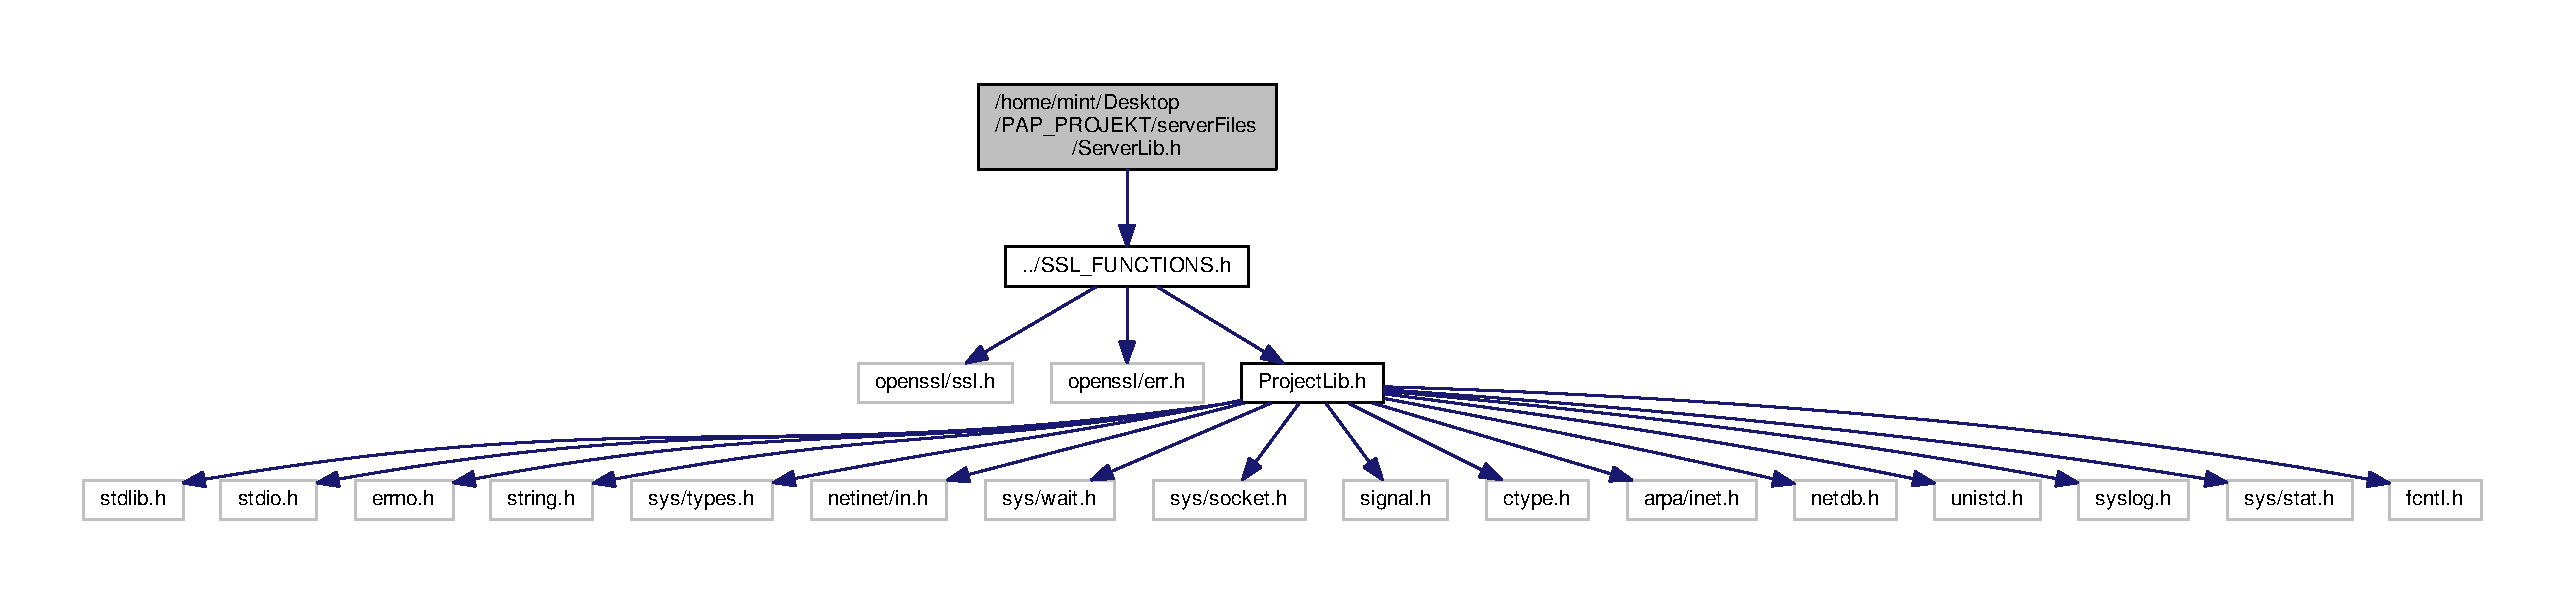
\includegraphics[width=350pt]{_server_lib_8h__incl}
\end{center}
\end{figure}
This graph shows which files directly or indirectly include this file\+:\nopagebreak
\begin{figure}[H]
\begin{center}
\leavevmode
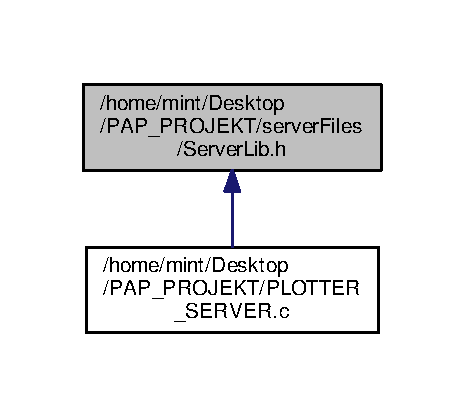
\includegraphics[width=223pt]{_server_lib_8h__dep__incl}
\end{center}
\end{figure}
\subsection*{Functions}
\begin{DoxyCompactItemize}
\item 
void \hyperlink{_server_lib_8h_aca4792f4c960c09ac7b39fd7edae2c16}{create\+Daemon} ()
\item 
static void \hyperlink{_server_lib_8h_aeb15c822259f5a1106af2bee31ee500b}{demonize} ()
\item 
static void \hyperlink{_server_lib_8h_a80c4cb425067dcd535ea2079e697014b}{log\+Server\+Notice} ()
\item 
void \hyperlink{_server_lib_8h_a40fdfd52c86ec3e5079b74b0533c7363}{Bind\+With\+Port\+And\+Run} (int \hyperlink{_p_l_o_t_t_e_r___s_e_r_v_e_r_8c_aeefbbafa97642defe3ee6c3080b7d66f}{B\+A\+C\+K\+L\+OG}, int \hyperlink{_p_l_o_t_t_e_r___s_e_r_v_e_r_8c_a614217d263be1fb1a5f76e2ff7be19a2}{P\+O\+RT})
\item 
static int \hyperlink{_server_lib_8h_a7a56f581ff1fd1820c4509ed7b9167b6}{Get\+Server\+Socket\+FD} ()
\item 
static void \hyperlink{_server_lib_8h_a48b48ace2f1c7517d46a92ca743a1f4f}{Listen\+To\+Remote} ()
\item 
static void \hyperlink{_server_lib_8h_a9674cd6c678554c56dfab098c4020fa7}{Obtain\+Connection} ()
\item 
static void \hyperlink{_server_lib_8h_a10923088fb087da55394f9a7e69b7925}{Receive\+File\+From\+Client} ()
\item 
static void \hyperlink{_server_lib_8h_ab997b2f7a1850edba0931b1fa359d937}{Create\+Plot} ()
\item 
static void \hyperlink{_server_lib_8h_a9ed99901d142c518bb99b28e3ef6702f}{Send\+Plot\+To\+Client} ()
\item 
static void \hyperlink{_server_lib_8h_af21a57de9f5a4e3fbc99ed1287032ab7}{Close\+Connection} ()
\item 
static void \hyperlink{_server_lib_8h_a7f98f17c443f1397d9a056e32a093229}{sigint\+Handler} ()
\end{DoxyCompactItemize}
\subsection*{Variables}
\begin{DoxyCompactItemize}
\item 
char $\ast$ \hyperlink{_server_lib_8h_a136e211133c7af859abfc129f4e950fa}{fr\+\_\+name} = \char`\"{}tmp/Plotter\+Server\+Files/receive.\+dat\char`\"{}
\begin{DoxyCompactList}\small\item\em Defines the localization of \textquotesingle{}receive.\+dat\textquotesingle{}. \end{DoxyCompactList}\item 
char $\ast$ \hyperlink{_server_lib_8h_ad5334765c4af576144103e5bfea9b01e}{fs\+\_\+name} = \char`\"{}tmp/Plotter\+Server\+Files/output.\+plt\char`\"{}
\begin{DoxyCompactList}\small\item\em Defines the localization of \textquotesingle{}output.\+plt\textquotesingle{}. \end{DoxyCompactList}\item 
char $\ast$ \hyperlink{_server_lib_8h_aaeebc6df5c6629080a763c0be580d74c}{plot\+Name} = \char`\"{}tmp/Plotter\+Server\+Files/output.\+png\char`\"{}
\begin{DoxyCompactList}\small\item\em Defines the localization of \textquotesingle{}output.\+png\textquotesingle{}. \end{DoxyCompactList}\item 
static char \hyperlink{_server_lib_8h_a3343eda9b3e780395a0509b3cd3c1cbd}{notice\+Buff} \mbox{[}256\mbox{]}
\begin{DoxyCompactList}\small\item\em The buffer of server notices. \end{DoxyCompactList}\item 
static int \hyperlink{_server_lib_8h_aaadb9a508ff3e162bdab7a45d54ce88e}{is\+Daemon} = 0
\begin{DoxyCompactList}\small\item\em Flag specifying whether server is a deamon. \end{DoxyCompactList}\item 
static int \hyperlink{_server_lib_8h_ad2c8fb3df3a737e0685e902870a611d2}{sockfd}
\begin{DoxyCompactList}\small\item\em Socket file descriptor. \end{DoxyCompactList}\item 
static int \hyperlink{_server_lib_8h_aa84798d04177520e38984d0234a64557}{nsockfd}
\begin{DoxyCompactList}\small\item\em New socket file descriptor. \end{DoxyCompactList}\item 
static int \hyperlink{_server_lib_8h_a9507e1c27beffe02ed97c7b076a42f24}{backlog}
\begin{DoxyCompactList}\small\item\em Defines the maximum length to which the queue of pending connections for sockfd. \end{DoxyCompactList}\item 
static int \hyperlink{_server_lib_8h_a63c89c04d1feae07ca35558055155ffb}{port}
\begin{DoxyCompactList}\small\item\em Server port number. \end{DoxyCompactList}\item 
static S\+S\+L\+\_\+\+M\+E\+T\+H\+OD $\ast$ \hyperlink{_server_lib_8h_a3557813aa116b56d10daf27b11a5f1e4}{server\+\_\+ssl\+\_\+method}
\begin{DoxyCompactList}\small\item\em Describes the ssl library functions which implement the protocol version. \end{DoxyCompactList}\item 
static S\+S\+L\+\_\+\+C\+TX $\ast$ \hyperlink{_server_lib_8h_a6565bf20bfe95e34576a921a32e2e844}{server\+\_\+ssl\+\_\+ctx}
\begin{DoxyCompactList}\small\item\em The global context structure. \end{DoxyCompactList}\item 
static S\+SL $\ast$ \hyperlink{_server_lib_8h_ae2dd01ac08721021386d7edf80ab31e8}{server\+\_\+ssl}
\begin{DoxyCompactList}\small\item\em Core structure in the S\+SL A\+PI. \end{DoxyCompactList}\end{DoxyCompactItemize}


\subsection{Function Documentation}
\index{Server\+Lib.\+h@{Server\+Lib.\+h}!Bind\+With\+Port\+And\+Run@{Bind\+With\+Port\+And\+Run}}
\index{Bind\+With\+Port\+And\+Run@{Bind\+With\+Port\+And\+Run}!Server\+Lib.\+h@{Server\+Lib.\+h}}
\subsubsection[{\texorpdfstring{Bind\+With\+Port\+And\+Run(int B\+A\+C\+K\+L\+O\+G, int P\+O\+R\+T)}{BindWithPortAndRun(int BACKLOG, int PORT)}}]{\setlength{\rightskip}{0pt plus 5cm}void Bind\+With\+Port\+And\+Run (
\begin{DoxyParamCaption}
\item[{int}]{B\+A\+C\+K\+L\+OG, }
\item[{int}]{P\+O\+RT}
\end{DoxyParamCaption}
)}\hypertarget{_server_lib_8h_a40fdfd52c86ec3e5079b74b0533c7363}{}\label{_server_lib_8h_a40fdfd52c86ec3e5079b74b0533c7363}
Binds server with port 

Definition at line 151 of file Server\+Lib.\+h.

\index{Server\+Lib.\+h@{Server\+Lib.\+h}!Close\+Connection@{Close\+Connection}}
\index{Close\+Connection@{Close\+Connection}!Server\+Lib.\+h@{Server\+Lib.\+h}}
\subsubsection[{\texorpdfstring{Close\+Connection()}{CloseConnection()}}]{\setlength{\rightskip}{0pt plus 5cm}static void Close\+Connection (
\begin{DoxyParamCaption}
{}
\end{DoxyParamCaption}
)\hspace{0.3cm}{\ttfamily [static]}}\hypertarget{_server_lib_8h_af21a57de9f5a4e3fbc99ed1287032ab7}{}\label{_server_lib_8h_af21a57de9f5a4e3fbc99ed1287032ab7}
Closes a connection with Client 

Definition at line 301 of file Server\+Lib.\+h.

\index{Server\+Lib.\+h@{Server\+Lib.\+h}!create\+Daemon@{create\+Daemon}}
\index{create\+Daemon@{create\+Daemon}!Server\+Lib.\+h@{Server\+Lib.\+h}}
\subsubsection[{\texorpdfstring{create\+Daemon()}{createDaemon()}}]{\setlength{\rightskip}{0pt plus 5cm}void create\+Daemon (
\begin{DoxyParamCaption}
{}
\end{DoxyParamCaption}
)}\hypertarget{_server_lib_8h_aca4792f4c960c09ac7b39fd7edae2c16}{}\label{_server_lib_8h_aca4792f4c960c09ac7b39fd7edae2c16}
Runs server as a daemon 

Definition at line 115 of file Server\+Lib.\+h.

\index{Server\+Lib.\+h@{Server\+Lib.\+h}!Create\+Plot@{Create\+Plot}}
\index{Create\+Plot@{Create\+Plot}!Server\+Lib.\+h@{Server\+Lib.\+h}}
\subsubsection[{\texorpdfstring{Create\+Plot()}{CreatePlot()}}]{\setlength{\rightskip}{0pt plus 5cm}static void Create\+Plot (
\begin{DoxyParamCaption}
{}
\end{DoxyParamCaption}
)\hspace{0.3cm}{\ttfamily [static]}}\hypertarget{_server_lib_8h_ab997b2f7a1850edba0931b1fa359d937}{}\label{_server_lib_8h_ab997b2f7a1850edba0931b1fa359d937}
Creates plot from data that the client has sent 

Definition at line 250 of file Server\+Lib.\+h.

\index{Server\+Lib.\+h@{Server\+Lib.\+h}!demonize@{demonize}}
\index{demonize@{demonize}!Server\+Lib.\+h@{Server\+Lib.\+h}}
\subsubsection[{\texorpdfstring{demonize()}{demonize()}}]{\setlength{\rightskip}{0pt plus 5cm}static void demonize (
\begin{DoxyParamCaption}
{}
\end{DoxyParamCaption}
)\hspace{0.3cm}{\ttfamily [static]}}\hypertarget{_server_lib_8h_aeb15c822259f5a1106af2bee31ee500b}{}\label{_server_lib_8h_aeb15c822259f5a1106af2bee31ee500b}
Creates daemon process 

Definition at line 48 of file Server\+Lib.\+h.

\index{Server\+Lib.\+h@{Server\+Lib.\+h}!Get\+Server\+Socket\+FD@{Get\+Server\+Socket\+FD}}
\index{Get\+Server\+Socket\+FD@{Get\+Server\+Socket\+FD}!Server\+Lib.\+h@{Server\+Lib.\+h}}
\subsubsection[{\texorpdfstring{Get\+Server\+Socket\+F\+D()}{GetServerSocketFD()}}]{\setlength{\rightskip}{0pt plus 5cm}int Get\+Server\+Socket\+FD (
\begin{DoxyParamCaption}
{}
\end{DoxyParamCaption}
)\hspace{0.3cm}{\ttfamily [static]}}\hypertarget{_server_lib_8h_a7a56f581ff1fd1820c4509ed7b9167b6}{}\label{_server_lib_8h_a7a56f581ff1fd1820c4509ed7b9167b6}
Return a socket file descriptor 

Definition at line 34 of file Server\+Lib.\+h.

\index{Server\+Lib.\+h@{Server\+Lib.\+h}!Listen\+To\+Remote@{Listen\+To\+Remote}}
\index{Listen\+To\+Remote@{Listen\+To\+Remote}!Server\+Lib.\+h@{Server\+Lib.\+h}}
\subsubsection[{\texorpdfstring{Listen\+To\+Remote()}{ListenToRemote()}}]{\setlength{\rightskip}{0pt plus 5cm}static void Listen\+To\+Remote (
\begin{DoxyParamCaption}
{}
\end{DoxyParamCaption}
)\hspace{0.3cm}{\ttfamily [static]}}\hypertarget{_server_lib_8h_a48b48ace2f1c7517d46a92ca743a1f4f}{}\label{_server_lib_8h_a48b48ace2f1c7517d46a92ca743a1f4f}
Listens to remote port 

Definition at line 185 of file Server\+Lib.\+h.

\index{Server\+Lib.\+h@{Server\+Lib.\+h}!log\+Server\+Notice@{log\+Server\+Notice}}
\index{log\+Server\+Notice@{log\+Server\+Notice}!Server\+Lib.\+h@{Server\+Lib.\+h}}
\subsubsection[{\texorpdfstring{log\+Server\+Notice()}{logServerNotice()}}]{\setlength{\rightskip}{0pt plus 5cm}static void log\+Server\+Notice (
\begin{DoxyParamCaption}
{}
\end{DoxyParamCaption}
)\hspace{0.3cm}{\ttfamily [static]}}\hypertarget{_server_lib_8h_a80c4cb425067dcd535ea2079e697014b}{}\label{_server_lib_8h_a80c4cb425067dcd535ea2079e697014b}
Logs servers notices 

Definition at line 126 of file Server\+Lib.\+h.

\index{Server\+Lib.\+h@{Server\+Lib.\+h}!Obtain\+Connection@{Obtain\+Connection}}
\index{Obtain\+Connection@{Obtain\+Connection}!Server\+Lib.\+h@{Server\+Lib.\+h}}
\subsubsection[{\texorpdfstring{Obtain\+Connection()}{ObtainConnection()}}]{\setlength{\rightskip}{0pt plus 5cm}static void Obtain\+Connection (
\begin{DoxyParamCaption}
{}
\end{DoxyParamCaption}
)\hspace{0.3cm}{\ttfamily [static]}}\hypertarget{_server_lib_8h_a9674cd6c678554c56dfab098c4020fa7}{}\label{_server_lib_8h_a9674cd6c678554c56dfab098c4020fa7}
Awaits connection and when one is established returns socket descriptor 

Definition at line 216 of file Server\+Lib.\+h.

\index{Server\+Lib.\+h@{Server\+Lib.\+h}!Receive\+File\+From\+Client@{Receive\+File\+From\+Client}}
\index{Receive\+File\+From\+Client@{Receive\+File\+From\+Client}!Server\+Lib.\+h@{Server\+Lib.\+h}}
\subsubsection[{\texorpdfstring{Receive\+File\+From\+Client()}{ReceiveFileFromClient()}}]{\setlength{\rightskip}{0pt plus 5cm}static void Receive\+File\+From\+Client (
\begin{DoxyParamCaption}
{}
\end{DoxyParamCaption}
)\hspace{0.3cm}{\ttfamily [static]}}\hypertarget{_server_lib_8h_a10923088fb087da55394f9a7e69b7925}{}\label{_server_lib_8h_a10923088fb087da55394f9a7e69b7925}
Receives file sent from client 

Definition at line 240 of file Server\+Lib.\+h.

\index{Server\+Lib.\+h@{Server\+Lib.\+h}!Send\+Plot\+To\+Client@{Send\+Plot\+To\+Client}}
\index{Send\+Plot\+To\+Client@{Send\+Plot\+To\+Client}!Server\+Lib.\+h@{Server\+Lib.\+h}}
\subsubsection[{\texorpdfstring{Send\+Plot\+To\+Client()}{SendPlotToClient()}}]{\setlength{\rightskip}{0pt plus 5cm}static void Send\+Plot\+To\+Client (
\begin{DoxyParamCaption}
{}
\end{DoxyParamCaption}
)\hspace{0.3cm}{\ttfamily [static]}}\hypertarget{_server_lib_8h_a9ed99901d142c518bb99b28e3ef6702f}{}\label{_server_lib_8h_a9ed99901d142c518bb99b28e3ef6702f}
Sends back a gnuplot in png format to the user 

Definition at line 290 of file Server\+Lib.\+h.

\index{Server\+Lib.\+h@{Server\+Lib.\+h}!sigint\+Handler@{sigint\+Handler}}
\index{sigint\+Handler@{sigint\+Handler}!Server\+Lib.\+h@{Server\+Lib.\+h}}
\subsubsection[{\texorpdfstring{sigint\+Handler()}{sigintHandler()}}]{\setlength{\rightskip}{0pt plus 5cm}static void sigint\+Handler (
\begin{DoxyParamCaption}
{}
\end{DoxyParamCaption}
)\hspace{0.3cm}{\ttfamily [static]}}\hypertarget{_server_lib_8h_a7f98f17c443f1397d9a056e32a093229}{}\label{_server_lib_8h_a7f98f17c443f1397d9a056e32a093229}
Handles S\+I\+G\+I\+NT, shuts down demon 

Definition at line 135 of file Server\+Lib.\+h.



\subsection{Variable Documentation}
\index{Server\+Lib.\+h@{Server\+Lib.\+h}!backlog@{backlog}}
\index{backlog@{backlog}!Server\+Lib.\+h@{Server\+Lib.\+h}}
\subsubsection[{\texorpdfstring{backlog}{backlog}}]{\setlength{\rightskip}{0pt plus 5cm}int backlog\hspace{0.3cm}{\ttfamily [static]}}\hypertarget{_server_lib_8h_a9507e1c27beffe02ed97c7b076a42f24}{}\label{_server_lib_8h_a9507e1c27beffe02ed97c7b076a42f24}


Defines the maximum length to which the queue of pending connections for sockfd. 



Definition at line 11 of file Server\+Lib.\+h.

\index{Server\+Lib.\+h@{Server\+Lib.\+h}!fr\+\_\+name@{fr\+\_\+name}}
\index{fr\+\_\+name@{fr\+\_\+name}!Server\+Lib.\+h@{Server\+Lib.\+h}}
\subsubsection[{\texorpdfstring{fr\+\_\+name}{fr_name}}]{\setlength{\rightskip}{0pt plus 5cm}char$\ast$ fr\+\_\+name = \char`\"{}tmp/Plotter\+Server\+Files/receive.\+dat\char`\"{}}\hypertarget{_server_lib_8h_a136e211133c7af859abfc129f4e950fa}{}\label{_server_lib_8h_a136e211133c7af859abfc129f4e950fa}


Defines the localization of \textquotesingle{}receive.\+dat\textquotesingle{}. 



Definition at line 3 of file Server\+Lib.\+h.

\index{Server\+Lib.\+h@{Server\+Lib.\+h}!fs\+\_\+name@{fs\+\_\+name}}
\index{fs\+\_\+name@{fs\+\_\+name}!Server\+Lib.\+h@{Server\+Lib.\+h}}
\subsubsection[{\texorpdfstring{fs\+\_\+name}{fs_name}}]{\setlength{\rightskip}{0pt plus 5cm}char$\ast$ fs\+\_\+name = \char`\"{}tmp/Plotter\+Server\+Files/output.\+plt\char`\"{}}\hypertarget{_server_lib_8h_ad5334765c4af576144103e5bfea9b01e}{}\label{_server_lib_8h_ad5334765c4af576144103e5bfea9b01e}


Defines the localization of \textquotesingle{}output.\+plt\textquotesingle{}. 



Definition at line 4 of file Server\+Lib.\+h.

\index{Server\+Lib.\+h@{Server\+Lib.\+h}!is\+Daemon@{is\+Daemon}}
\index{is\+Daemon@{is\+Daemon}!Server\+Lib.\+h@{Server\+Lib.\+h}}
\subsubsection[{\texorpdfstring{is\+Daemon}{isDaemon}}]{\setlength{\rightskip}{0pt plus 5cm}int is\+Daemon = 0\hspace{0.3cm}{\ttfamily [static]}}\hypertarget{_server_lib_8h_aaadb9a508ff3e162bdab7a45d54ce88e}{}\label{_server_lib_8h_aaadb9a508ff3e162bdab7a45d54ce88e}


Flag specifying whether server is a deamon. 



Definition at line 8 of file Server\+Lib.\+h.

\index{Server\+Lib.\+h@{Server\+Lib.\+h}!notice\+Buff@{notice\+Buff}}
\index{notice\+Buff@{notice\+Buff}!Server\+Lib.\+h@{Server\+Lib.\+h}}
\subsubsection[{\texorpdfstring{notice\+Buff}{noticeBuff}}]{\setlength{\rightskip}{0pt plus 5cm}char notice\+Buff\mbox{[}256\mbox{]}\hspace{0.3cm}{\ttfamily [static]}}\hypertarget{_server_lib_8h_a3343eda9b3e780395a0509b3cd3c1cbd}{}\label{_server_lib_8h_a3343eda9b3e780395a0509b3cd3c1cbd}


The buffer of server notices. 



Definition at line 7 of file Server\+Lib.\+h.

\index{Server\+Lib.\+h@{Server\+Lib.\+h}!nsockfd@{nsockfd}}
\index{nsockfd@{nsockfd}!Server\+Lib.\+h@{Server\+Lib.\+h}}
\subsubsection[{\texorpdfstring{nsockfd}{nsockfd}}]{\setlength{\rightskip}{0pt plus 5cm}int nsockfd\hspace{0.3cm}{\ttfamily [static]}}\hypertarget{_server_lib_8h_aa84798d04177520e38984d0234a64557}{}\label{_server_lib_8h_aa84798d04177520e38984d0234a64557}


New socket file descriptor. 



Definition at line 10 of file Server\+Lib.\+h.

\index{Server\+Lib.\+h@{Server\+Lib.\+h}!plot\+Name@{plot\+Name}}
\index{plot\+Name@{plot\+Name}!Server\+Lib.\+h@{Server\+Lib.\+h}}
\subsubsection[{\texorpdfstring{plot\+Name}{plotName}}]{\setlength{\rightskip}{0pt plus 5cm}char$\ast$ plot\+Name = \char`\"{}tmp/Plotter\+Server\+Files/output.\+png\char`\"{}}\hypertarget{_server_lib_8h_aaeebc6df5c6629080a763c0be580d74c}{}\label{_server_lib_8h_aaeebc6df5c6629080a763c0be580d74c}


Defines the localization of \textquotesingle{}output.\+png\textquotesingle{}. 



Definition at line 5 of file Server\+Lib.\+h.

\index{Server\+Lib.\+h@{Server\+Lib.\+h}!port@{port}}
\index{port@{port}!Server\+Lib.\+h@{Server\+Lib.\+h}}
\subsubsection[{\texorpdfstring{port}{port}}]{\setlength{\rightskip}{0pt plus 5cm}int port\hspace{0.3cm}{\ttfamily [static]}}\hypertarget{_server_lib_8h_a63c89c04d1feae07ca35558055155ffb}{}\label{_server_lib_8h_a63c89c04d1feae07ca35558055155ffb}


Server port number. 



Definition at line 12 of file Server\+Lib.\+h.

\index{Server\+Lib.\+h@{Server\+Lib.\+h}!server\+\_\+ssl@{server\+\_\+ssl}}
\index{server\+\_\+ssl@{server\+\_\+ssl}!Server\+Lib.\+h@{Server\+Lib.\+h}}
\subsubsection[{\texorpdfstring{server\+\_\+ssl}{server_ssl}}]{\setlength{\rightskip}{0pt plus 5cm}S\+SL$\ast$ server\+\_\+ssl\hspace{0.3cm}{\ttfamily [static]}}\hypertarget{_server_lib_8h_ae2dd01ac08721021386d7edf80ab31e8}{}\label{_server_lib_8h_ae2dd01ac08721021386d7edf80ab31e8}


Core structure in the S\+SL A\+PI. 



Definition at line 16 of file Server\+Lib.\+h.

\index{Server\+Lib.\+h@{Server\+Lib.\+h}!server\+\_\+ssl\+\_\+ctx@{server\+\_\+ssl\+\_\+ctx}}
\index{server\+\_\+ssl\+\_\+ctx@{server\+\_\+ssl\+\_\+ctx}!Server\+Lib.\+h@{Server\+Lib.\+h}}
\subsubsection[{\texorpdfstring{server\+\_\+ssl\+\_\+ctx}{server_ssl_ctx}}]{\setlength{\rightskip}{0pt plus 5cm}S\+S\+L\+\_\+\+C\+TX$\ast$ server\+\_\+ssl\+\_\+ctx\hspace{0.3cm}{\ttfamily [static]}}\hypertarget{_server_lib_8h_a6565bf20bfe95e34576a921a32e2e844}{}\label{_server_lib_8h_a6565bf20bfe95e34576a921a32e2e844}


The global context structure. 



Definition at line 15 of file Server\+Lib.\+h.

\index{Server\+Lib.\+h@{Server\+Lib.\+h}!server\+\_\+ssl\+\_\+method@{server\+\_\+ssl\+\_\+method}}
\index{server\+\_\+ssl\+\_\+method@{server\+\_\+ssl\+\_\+method}!Server\+Lib.\+h@{Server\+Lib.\+h}}
\subsubsection[{\texorpdfstring{server\+\_\+ssl\+\_\+method}{server_ssl_method}}]{\setlength{\rightskip}{0pt plus 5cm}S\+S\+L\+\_\+\+M\+E\+T\+H\+OD$\ast$ server\+\_\+ssl\+\_\+method\hspace{0.3cm}{\ttfamily [static]}}\hypertarget{_server_lib_8h_a3557813aa116b56d10daf27b11a5f1e4}{}\label{_server_lib_8h_a3557813aa116b56d10daf27b11a5f1e4}


Describes the ssl library functions which implement the protocol version. 



Definition at line 14 of file Server\+Lib.\+h.

\index{Server\+Lib.\+h@{Server\+Lib.\+h}!sockfd@{sockfd}}
\index{sockfd@{sockfd}!Server\+Lib.\+h@{Server\+Lib.\+h}}
\subsubsection[{\texorpdfstring{sockfd}{sockfd}}]{\setlength{\rightskip}{0pt plus 5cm}int sockfd\hspace{0.3cm}{\ttfamily [static]}}\hypertarget{_server_lib_8h_ad2c8fb3df3a737e0685e902870a611d2}{}\label{_server_lib_8h_ad2c8fb3df3a737e0685e902870a611d2}


Socket file descriptor. 



Definition at line 9 of file Server\+Lib.\+h.


\hypertarget{_s_s_l___f_u_n_c_t_i_o_n_s_8h}{}\section{/home/mint/\+Desktop/\+P\+A\+P\+\_\+\+P\+R\+O\+J\+E\+K\+T/\+S\+S\+L\+\_\+\+F\+U\+N\+C\+T\+I\+O\+NS.h File Reference}
\label{_s_s_l___f_u_n_c_t_i_o_n_s_8h}\index{/home/mint/\+Desktop/\+P\+A\+P\+\_\+\+P\+R\+O\+J\+E\+K\+T/\+S\+S\+L\+\_\+\+F\+U\+N\+C\+T\+I\+O\+N\+S.\+h@{/home/mint/\+Desktop/\+P\+A\+P\+\_\+\+P\+R\+O\+J\+E\+K\+T/\+S\+S\+L\+\_\+\+F\+U\+N\+C\+T\+I\+O\+N\+S.\+h}}
{\ttfamily \#include $<$openssl/ssl.\+h$>$}\\*
{\ttfamily \#include $<$openssl/err.\+h$>$}\\*
{\ttfamily \#include \char`\"{}Project\+Lib.\+h\char`\"{}}\\*
Include dependency graph for S\+S\+L\+\_\+\+F\+U\+N\+C\+T\+I\+O\+N\+S.\+h\+:\nopagebreak
\begin{figure}[H]
\begin{center}
\leavevmode
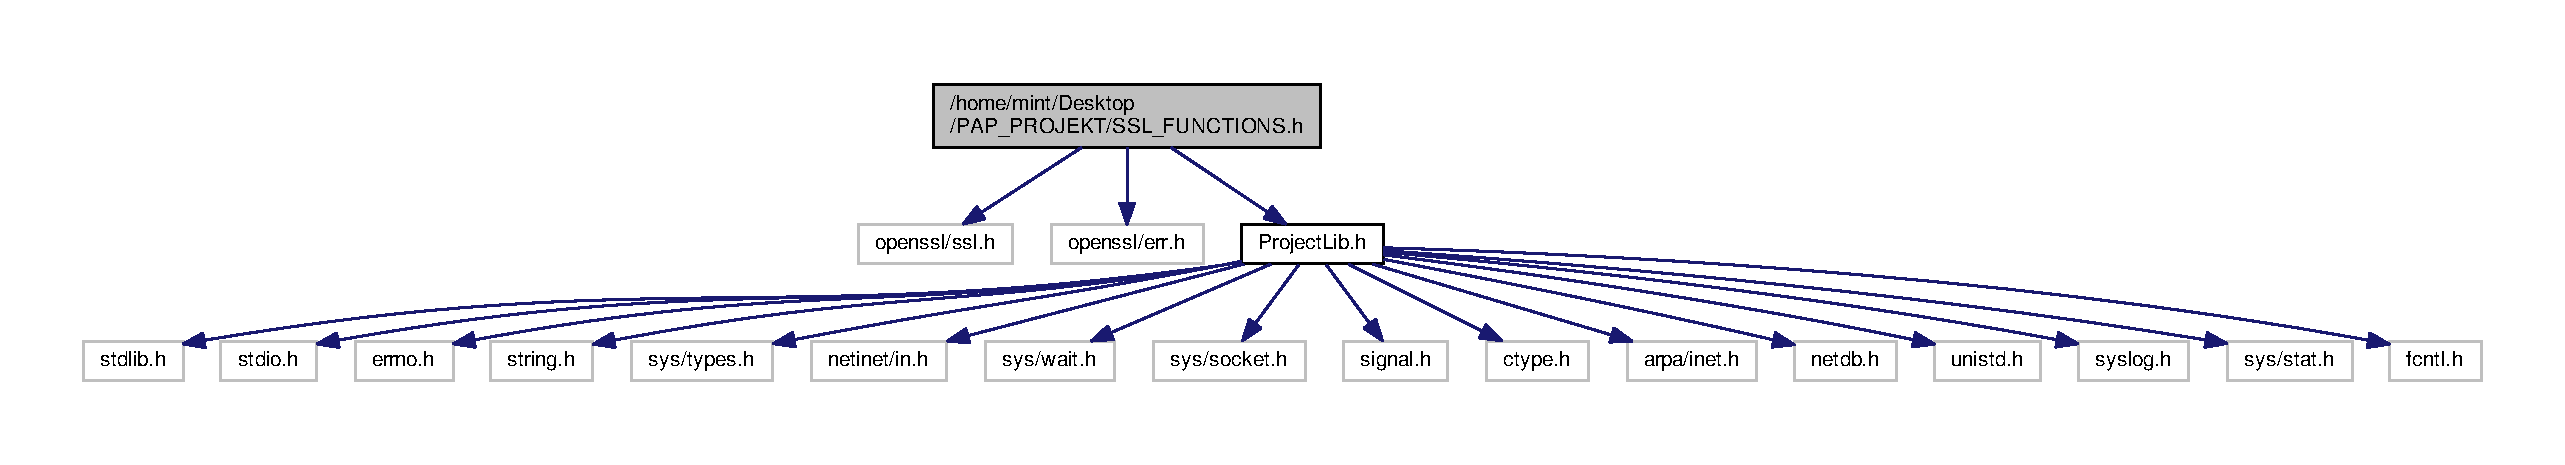
\includegraphics[width=350pt]{_s_s_l___f_u_n_c_t_i_o_n_s_8h__incl}
\end{center}
\end{figure}
This graph shows which files directly or indirectly include this file\+:\nopagebreak
\begin{figure}[H]
\begin{center}
\leavevmode
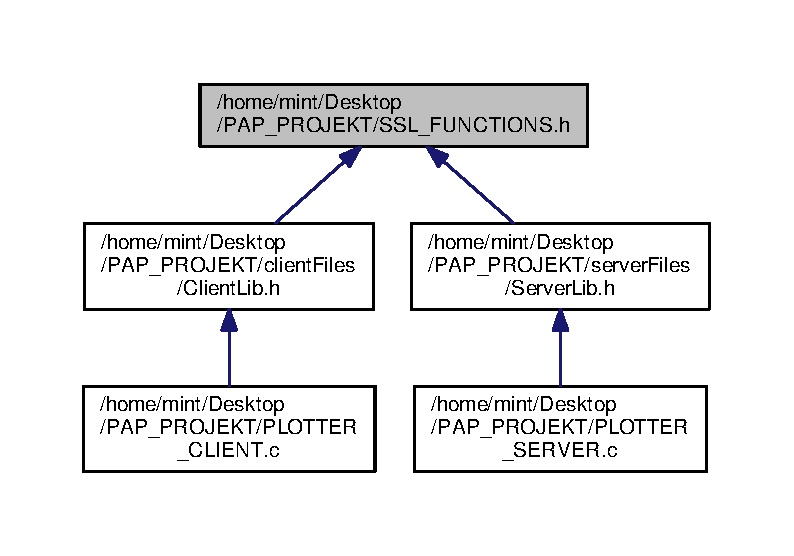
\includegraphics[width=350pt]{_s_s_l___f_u_n_c_t_i_o_n_s_8h__dep__incl}
\end{center}
\end{figure}
\subsection*{Functions}
\begin{DoxyCompactItemize}
\item 
void \hyperlink{_s_s_l___f_u_n_c_t_i_o_n_s_8h_ac9bc33eb715effb434f721bf1fb1fd2f}{S\+S\+L\+F\+\_\+\+Init\+Server} (S\+S\+L\+\_\+\+M\+E\+T\+H\+OD $\ast$$\ast$\hyperlink{_server_lib_8h_a3557813aa116b56d10daf27b11a5f1e4}{server\+\_\+ssl\+\_\+method}, S\+S\+L\+\_\+\+C\+TX $\ast$$\ast$\hyperlink{_server_lib_8h_a6565bf20bfe95e34576a921a32e2e844}{server\+\_\+ssl\+\_\+ctx})
\item 
void \hyperlink{_s_s_l___f_u_n_c_t_i_o_n_s_8h_ab8ceaea88e54727c8ac4d4540cf4f28f}{S\+S\+L\+F\+\_\+\+Accept\+Connection} (S\+SL $\ast$$\ast$\hyperlink{_server_lib_8h_ae2dd01ac08721021386d7edf80ab31e8}{server\+\_\+ssl}, S\+S\+L\+\_\+\+C\+TX $\ast$\hyperlink{_server_lib_8h_a6565bf20bfe95e34576a921a32e2e844}{server\+\_\+ssl\+\_\+ctx}, int \hyperlink{_server_lib_8h_aa84798d04177520e38984d0234a64557}{nsockfd})
\item 
void \hyperlink{_s_s_l___f_u_n_c_t_i_o_n_s_8h_a4348638952bd3323328bc453df933767}{S\+S\+L\+F\+\_\+\+Init\+Client} (S\+S\+L\+\_\+\+M\+E\+T\+H\+OD $\ast$$\ast$\hyperlink{_client_lib_8h_a67a0b3150dfacb2f75fba66e0959f560}{client\+\_\+ssl\+\_\+method}, S\+S\+L\+\_\+\+C\+TX $\ast$$\ast$\hyperlink{_client_lib_8h_ae5429a87dee8628ab5a51bdcb88e336a}{client\+\_\+ssl\+\_\+ctx}, S\+SL $\ast$$\ast$\hyperlink{_client_lib_8h_a29a4fb7a75bd99073cdf6a6c871ad771}{client\+\_\+ssl})
\item 
void \hyperlink{_s_s_l___f_u_n_c_t_i_o_n_s_8h_a8e8bb741e8f7385da02df44acc221fed}{S\+S\+L\+F\+\_\+\+Connect\+With\+Server} (S\+SL $\ast$\hyperlink{_client_lib_8h_a29a4fb7a75bd99073cdf6a6c871ad771}{client\+\_\+ssl}, int \hyperlink{_server_lib_8h_ad2c8fb3df3a737e0685e902870a611d2}{sockfd})
\item 
void \hyperlink{_s_s_l___f_u_n_c_t_i_o_n_s_8h_a4bf96901c24e8b3ef29150ff9ffbc38f}{S\+S\+L\+F\+\_\+\+Recieve\+Big\+And\+Save} (S\+SL $\ast$source, char $\ast$Save\+As)
\item 
void \hyperlink{_s_s_l___f_u_n_c_t_i_o_n_s_8h_a964050927869014e690d941a64f1e178}{S\+S\+L\+F\+\_\+\+Recieve\+Small\+And\+Save} (S\+SL $\ast$source, char $\ast$Save\+As)
\item 
void \hyperlink{_s_s_l___f_u_n_c_t_i_o_n_s_8h_a9071bc242ebce480973a3e82e29de061}{S\+S\+L\+F\+\_\+\+Open\+And\+Send} (S\+SL $\ast$sink, char $\ast$From\+File)
\end{DoxyCompactItemize}


\subsection{Function Documentation}
\index{S\+S\+L\+\_\+\+F\+U\+N\+C\+T\+I\+O\+N\+S.\+h@{S\+S\+L\+\_\+\+F\+U\+N\+C\+T\+I\+O\+N\+S.\+h}!S\+S\+L\+F\+\_\+\+Accept\+Connection@{S\+S\+L\+F\+\_\+\+Accept\+Connection}}
\index{S\+S\+L\+F\+\_\+\+Accept\+Connection@{S\+S\+L\+F\+\_\+\+Accept\+Connection}!S\+S\+L\+\_\+\+F\+U\+N\+C\+T\+I\+O\+N\+S.\+h@{S\+S\+L\+\_\+\+F\+U\+N\+C\+T\+I\+O\+N\+S.\+h}}
\subsubsection[{\texorpdfstring{S\+S\+L\+F\+\_\+\+Accept\+Connection(\+S\+S\+L $\ast$$\ast$server\+\_\+ssl, S\+S\+L\+\_\+\+C\+T\+X $\ast$server\+\_\+ssl\+\_\+ctx, int nsockfd)}{SSLF_AcceptConnection(SSL **server_ssl, SSL_CTX *server_ssl_ctx, int nsockfd)}}]{\setlength{\rightskip}{0pt plus 5cm}void S\+S\+L\+F\+\_\+\+Accept\+Connection (
\begin{DoxyParamCaption}
\item[{S\+SL $\ast$$\ast$}]{server\+\_\+ssl, }
\item[{S\+S\+L\+\_\+\+C\+TX $\ast$}]{server\+\_\+ssl\+\_\+ctx, }
\item[{int}]{nsockfd}
\end{DoxyParamCaption}
)}\hypertarget{_s_s_l___f_u_n_c_t_i_o_n_s_8h_ab8ceaea88e54727c8ac4d4540cf4f28f}{}\label{_s_s_l___f_u_n_c_t_i_o_n_s_8h_ab8ceaea88e54727c8ac4d4540cf4f28f}
Connects server with a socket file descriptor 

Definition at line 41 of file S\+S\+L\+\_\+\+F\+U\+N\+C\+T\+I\+O\+N\+S.\+h.

\index{S\+S\+L\+\_\+\+F\+U\+N\+C\+T\+I\+O\+N\+S.\+h@{S\+S\+L\+\_\+\+F\+U\+N\+C\+T\+I\+O\+N\+S.\+h}!S\+S\+L\+F\+\_\+\+Connect\+With\+Server@{S\+S\+L\+F\+\_\+\+Connect\+With\+Server}}
\index{S\+S\+L\+F\+\_\+\+Connect\+With\+Server@{S\+S\+L\+F\+\_\+\+Connect\+With\+Server}!S\+S\+L\+\_\+\+F\+U\+N\+C\+T\+I\+O\+N\+S.\+h@{S\+S\+L\+\_\+\+F\+U\+N\+C\+T\+I\+O\+N\+S.\+h}}
\subsubsection[{\texorpdfstring{S\+S\+L\+F\+\_\+\+Connect\+With\+Server(\+S\+S\+L $\ast$client\+\_\+ssl, int sockfd)}{SSLF_ConnectWithServer(SSL *client_ssl, int sockfd)}}]{\setlength{\rightskip}{0pt plus 5cm}void S\+S\+L\+F\+\_\+\+Connect\+With\+Server (
\begin{DoxyParamCaption}
\item[{S\+SL $\ast$}]{client\+\_\+ssl, }
\item[{int}]{sockfd}
\end{DoxyParamCaption}
)}\hypertarget{_s_s_l___f_u_n_c_t_i_o_n_s_8h_a8e8bb741e8f7385da02df44acc221fed}{}\label{_s_s_l___f_u_n_c_t_i_o_n_s_8h_a8e8bb741e8f7385da02df44acc221fed}
Connects client to server 

Definition at line 88 of file S\+S\+L\+\_\+\+F\+U\+N\+C\+T\+I\+O\+N\+S.\+h.

\index{S\+S\+L\+\_\+\+F\+U\+N\+C\+T\+I\+O\+N\+S.\+h@{S\+S\+L\+\_\+\+F\+U\+N\+C\+T\+I\+O\+N\+S.\+h}!S\+S\+L\+F\+\_\+\+Init\+Client@{S\+S\+L\+F\+\_\+\+Init\+Client}}
\index{S\+S\+L\+F\+\_\+\+Init\+Client@{S\+S\+L\+F\+\_\+\+Init\+Client}!S\+S\+L\+\_\+\+F\+U\+N\+C\+T\+I\+O\+N\+S.\+h@{S\+S\+L\+\_\+\+F\+U\+N\+C\+T\+I\+O\+N\+S.\+h}}
\subsubsection[{\texorpdfstring{S\+S\+L\+F\+\_\+\+Init\+Client(\+S\+S\+L\+\_\+\+M\+E\+T\+H\+O\+D $\ast$$\ast$client\+\_\+ssl\+\_\+method, S\+S\+L\+\_\+\+C\+T\+X $\ast$$\ast$client\+\_\+ssl\+\_\+ctx, S\+S\+L $\ast$$\ast$client\+\_\+ssl)}{SSLF_InitClient(SSL_METHOD **client_ssl_method, SSL_CTX **client_ssl_ctx, SSL **client_ssl)}}]{\setlength{\rightskip}{0pt plus 5cm}void S\+S\+L\+F\+\_\+\+Init\+Client (
\begin{DoxyParamCaption}
\item[{S\+S\+L\+\_\+\+M\+E\+T\+H\+OD $\ast$$\ast$}]{client\+\_\+ssl\+\_\+method, }
\item[{S\+S\+L\+\_\+\+C\+TX $\ast$$\ast$}]{client\+\_\+ssl\+\_\+ctx, }
\item[{S\+SL $\ast$$\ast$}]{client\+\_\+ssl}
\end{DoxyParamCaption}
)}\hypertarget{_s_s_l___f_u_n_c_t_i_o_n_s_8h_a4348638952bd3323328bc453df933767}{}\label{_s_s_l___f_u_n_c_t_i_o_n_s_8h_a4348638952bd3323328bc453df933767}
Sets up S\+SL for client 

Definition at line 64 of file S\+S\+L\+\_\+\+F\+U\+N\+C\+T\+I\+O\+N\+S.\+h.

\index{S\+S\+L\+\_\+\+F\+U\+N\+C\+T\+I\+O\+N\+S.\+h@{S\+S\+L\+\_\+\+F\+U\+N\+C\+T\+I\+O\+N\+S.\+h}!S\+S\+L\+F\+\_\+\+Init\+Server@{S\+S\+L\+F\+\_\+\+Init\+Server}}
\index{S\+S\+L\+F\+\_\+\+Init\+Server@{S\+S\+L\+F\+\_\+\+Init\+Server}!S\+S\+L\+\_\+\+F\+U\+N\+C\+T\+I\+O\+N\+S.\+h@{S\+S\+L\+\_\+\+F\+U\+N\+C\+T\+I\+O\+N\+S.\+h}}
\subsubsection[{\texorpdfstring{S\+S\+L\+F\+\_\+\+Init\+Server(\+S\+S\+L\+\_\+\+M\+E\+T\+H\+O\+D $\ast$$\ast$server\+\_\+ssl\+\_\+method, S\+S\+L\+\_\+\+C\+T\+X $\ast$$\ast$server\+\_\+ssl\+\_\+ctx)}{SSLF_InitServer(SSL_METHOD **server_ssl_method, SSL_CTX **server_ssl_ctx)}}]{\setlength{\rightskip}{0pt plus 5cm}void S\+S\+L\+F\+\_\+\+Init\+Server (
\begin{DoxyParamCaption}
\item[{S\+S\+L\+\_\+\+M\+E\+T\+H\+OD $\ast$$\ast$}]{server\+\_\+ssl\+\_\+method, }
\item[{S\+S\+L\+\_\+\+C\+TX $\ast$$\ast$}]{server\+\_\+ssl\+\_\+ctx}
\end{DoxyParamCaption}
)}\hypertarget{_s_s_l___f_u_n_c_t_i_o_n_s_8h_ac9bc33eb715effb434f721bf1fb1fd2f}{}\label{_s_s_l___f_u_n_c_t_i_o_n_s_8h_ac9bc33eb715effb434f721bf1fb1fd2f}
Set up S\+SL for server 

Definition at line 16 of file S\+S\+L\+\_\+\+F\+U\+N\+C\+T\+I\+O\+N\+S.\+h.

\index{S\+S\+L\+\_\+\+F\+U\+N\+C\+T\+I\+O\+N\+S.\+h@{S\+S\+L\+\_\+\+F\+U\+N\+C\+T\+I\+O\+N\+S.\+h}!S\+S\+L\+F\+\_\+\+Open\+And\+Send@{S\+S\+L\+F\+\_\+\+Open\+And\+Send}}
\index{S\+S\+L\+F\+\_\+\+Open\+And\+Send@{S\+S\+L\+F\+\_\+\+Open\+And\+Send}!S\+S\+L\+\_\+\+F\+U\+N\+C\+T\+I\+O\+N\+S.\+h@{S\+S\+L\+\_\+\+F\+U\+N\+C\+T\+I\+O\+N\+S.\+h}}
\subsubsection[{\texorpdfstring{S\+S\+L\+F\+\_\+\+Open\+And\+Send(\+S\+S\+L $\ast$sink, char $\ast$\+From\+File)}{SSLF_OpenAndSend(SSL *sink, char *FromFile)}}]{\setlength{\rightskip}{0pt plus 5cm}void S\+S\+L\+F\+\_\+\+Open\+And\+Send (
\begin{DoxyParamCaption}
\item[{S\+SL $\ast$}]{sink, }
\item[{char $\ast$}]{From\+File}
\end{DoxyParamCaption}
)}\hypertarget{_s_s_l___f_u_n_c_t_i_o_n_s_8h_a9071bc242ebce480973a3e82e29de061}{}\label{_s_s_l___f_u_n_c_t_i_o_n_s_8h_a9071bc242ebce480973a3e82e29de061}
Sends file 

Definition at line 147 of file S\+S\+L\+\_\+\+F\+U\+N\+C\+T\+I\+O\+N\+S.\+h.

\index{S\+S\+L\+\_\+\+F\+U\+N\+C\+T\+I\+O\+N\+S.\+h@{S\+S\+L\+\_\+\+F\+U\+N\+C\+T\+I\+O\+N\+S.\+h}!S\+S\+L\+F\+\_\+\+Recieve\+Big\+And\+Save@{S\+S\+L\+F\+\_\+\+Recieve\+Big\+And\+Save}}
\index{S\+S\+L\+F\+\_\+\+Recieve\+Big\+And\+Save@{S\+S\+L\+F\+\_\+\+Recieve\+Big\+And\+Save}!S\+S\+L\+\_\+\+F\+U\+N\+C\+T\+I\+O\+N\+S.\+h@{S\+S\+L\+\_\+\+F\+U\+N\+C\+T\+I\+O\+N\+S.\+h}}
\subsubsection[{\texorpdfstring{S\+S\+L\+F\+\_\+\+Recieve\+Big\+And\+Save(\+S\+S\+L $\ast$source, char $\ast$\+Save\+As)}{SSLF_RecieveBigAndSave(SSL *source, char *SaveAs)}}]{\setlength{\rightskip}{0pt plus 5cm}void S\+S\+L\+F\+\_\+\+Recieve\+Big\+And\+Save (
\begin{DoxyParamCaption}
\item[{S\+SL $\ast$}]{source, }
\item[{char $\ast$}]{Save\+As}
\end{DoxyParamCaption}
)}\hypertarget{_s_s_l___f_u_n_c_t_i_o_n_s_8h_a4bf96901c24e8b3ef29150ff9ffbc38f}{}\label{_s_s_l___f_u_n_c_t_i_o_n_s_8h_a4bf96901c24e8b3ef29150ff9ffbc38f}
Reads recived bytes (larger files) and save them 

Definition at line 102 of file S\+S\+L\+\_\+\+F\+U\+N\+C\+T\+I\+O\+N\+S.\+h.

\index{S\+S\+L\+\_\+\+F\+U\+N\+C\+T\+I\+O\+N\+S.\+h@{S\+S\+L\+\_\+\+F\+U\+N\+C\+T\+I\+O\+N\+S.\+h}!S\+S\+L\+F\+\_\+\+Recieve\+Small\+And\+Save@{S\+S\+L\+F\+\_\+\+Recieve\+Small\+And\+Save}}
\index{S\+S\+L\+F\+\_\+\+Recieve\+Small\+And\+Save@{S\+S\+L\+F\+\_\+\+Recieve\+Small\+And\+Save}!S\+S\+L\+\_\+\+F\+U\+N\+C\+T\+I\+O\+N\+S.\+h@{S\+S\+L\+\_\+\+F\+U\+N\+C\+T\+I\+O\+N\+S.\+h}}
\subsubsection[{\texorpdfstring{S\+S\+L\+F\+\_\+\+Recieve\+Small\+And\+Save(\+S\+S\+L $\ast$source, char $\ast$\+Save\+As)}{SSLF_RecieveSmallAndSave(SSL *source, char *SaveAs)}}]{\setlength{\rightskip}{0pt plus 5cm}void S\+S\+L\+F\+\_\+\+Recieve\+Small\+And\+Save (
\begin{DoxyParamCaption}
\item[{S\+SL $\ast$}]{source, }
\item[{char $\ast$}]{Save\+As}
\end{DoxyParamCaption}
)}\hypertarget{_s_s_l___f_u_n_c_t_i_o_n_s_8h_a964050927869014e690d941a64f1e178}{}\label{_s_s_l___f_u_n_c_t_i_o_n_s_8h_a964050927869014e690d941a64f1e178}
Reads recived bytes and save them 

Definition at line 123 of file S\+S\+L\+\_\+\+F\+U\+N\+C\+T\+I\+O\+N\+S.\+h.


%--- End generated contents ---

% Index
\backmatter
\newpage
\phantomsection
\clearemptydoublepage
\addcontentsline{toc}{chapter}{Index}
\printindex

\end{document}
